% !TeX program = xelatex
\documentclass[11pt,a4paper]{article}

% -------------------------------------------------
% Packages
% -------------------------------------------------
\usepackage{kotex}
\usepackage{fontspec}
\usepackage{amsmath,amssymb,bm,mathtools}
\usepackage[left=24mm,right=24mm,top=23mm,bottom=25mm]{geometry}
\usepackage{booktabs,array}
\usepackage{enumitem}
\usepackage{setspace}
\usepackage{xcolor}
\usepackage{colortbl}
\usepackage{graphicx}
\usepackage{tikz}
\usepackage{pifont}
\usetikzlibrary{positioning,arrows.meta,calc,fit,decorations.pathreplacing,shapes.geometric}
\usepackage[most]{tcolorbox}
\usepackage{listings}
\usepackage{hyperref}
\usepackage{fancyhdr}

\setstretch{1.14}
\setlength{\parindent}{0pt}
\setlength{\parskip}{0.55em}
\setlength{\emergencystretch}{2em}   % long \texttt{...} words: stretch the line instead of overfull

% -------------------------------------------------
% Colors and boxes
% -------------------------------------------------
\definecolor{deepblue}{RGB}{34,71,120}
\definecolor{softblue}{RGB}{239,246,253}
\definecolor{softgray}{RGB}{246,247,249}
\definecolor{softgreen}{RGB}{239,249,242}
\definecolor{softyellow}{RGB}{255,249,229}
\definecolor{codegray}{RGB}{248,248,248}

\newtcolorbox{keybox}[1][]{
  colback=softblue,
  colframe=deepblue,
  boxrule=0.7pt,
  arc=2mm,
  title=#1,
  fonttitle=\bfseries
}

\newtcolorbox{thinkbox}[1][]{
  colback=softyellow,
  colframe=orange!70!black,
  boxrule=0.6pt,
  arc=2mm,
  title=#1,
  fonttitle=\bfseries
}

\newtcolorbox{remarkbox}[1][]{
  colback=softgray,
  colframe=black!45,
  boxrule=0.5pt,
  arc=2mm,
  title=#1,
  fonttitle=\bfseries
}

\newtcolorbox{mlbox}[1][]{
  colback=softgreen,
  colframe=green!45!black,
  boxrule=0.6pt,
  arc=2mm,
  title=#1,
  fonttitle=\bfseries
}

% -------------------------------------------------
% Code style
% -------------------------------------------------
\lstdefinestyle{pythonstyle}{
  language=Python,
  backgroundcolor=\color{codegray},
  basicstyle=\ttfamily\small,
  keywordstyle=\bfseries,
  commentstyle=\itshape\color{black!60},
  stringstyle=\color{black!75},
  numbers=left,
  numberstyle=\tiny\color{black!55},
  numbersep=8pt,
  frame=single,
  rulecolor=\color{black!25},
  breaklines=true,
  showstringspaces=false,
  tabsize=4,
  columns=fullflexible,
  keepspaces=true
}
\lstset{style=pythonstyle}

% -------------------------------------------------
% Math commands
% -------------------------------------------------
\newcommand{\R}{\mathbb{R}}
\newcommand{\grad}{\nabla}
\newcommand{\vect}[1]{\bm{#1}}
\newcommand{\T}{^{\mathsf T}}
\newcommand{\loss}{\mathcal{L}}
\newcommand{\pd}[2]{\frac{\partial #1}{\partial #2}}
\newcommand{\softmax}{\operatorname{softmax}}

% -------------------------------------------------
% Header / footer
% -------------------------------------------------
\pagestyle{fancy}
\fancyhf{}
\lhead{Introduction to Deep Learning and Practice}
\rhead{Deep Learning}
\cfoot{\thepage}
\renewcommand{\headrulewidth}{0.4pt}
\setlength{\headheight}{14pt}

\hypersetup{
  colorlinks=true,
  linkcolor=deepblue,
  urlcolor=deepblue
}

% =================================================
% =================================================
\begin{document}
% =================================================

\begin{center}
{\LARGE\bfseries 딥러닝 (Deep Learning)}\\[0.35em]
{\large 더 깊은 CNN $\cdot$ ImageNet과 대표 신경망 $\cdot$ 고속화 $\cdot$ 활용과 미래}\\[0.8em]
\end{center}

\vspace{0.4em}

\begin{keybox}[이번 주의 핵심 질문]
\textbf{딥러닝}은 층을 깊게 쌓은 신경망이다. 지금까지 만든 신경망은 은닉층이 한두 개였다.
층을 더 깊게 쌓으면 무엇이 좋아지고, 어떤 어려움이 생기는가?
그리고 2012년부터 2015년까지 단 몇 년 사이에 이미지 인식의 오류율이 사람 수준 아래로 떨어졌는데,
그동안 무엇이 바뀌었는가?
\end{keybox}

\subsection*{학습목표}

이 주차가 끝나면 다음을 설명할 수 있어야 한다.

\begin{enumerate}[label=\arabic*.]
\item 합성곱 계층 $6$개로 된 DeepConvNet의 구조를 각 계층의 shape과 매개변수 수로 설명한다.
\item 데이터 확장(data augmentation)의 방법과 효과를 설명한다.
\item 층을 깊게 하는 이점 (적은 매개변수, 넓은 수용 영역, 많은 비선형성, 계층적 학습)을 계산으로 보인다.
\item ImageNet 대회의 흐름과 VGG, GoogLeNet ($1\times1$ 합성곱), ResNet (skip connection)의 핵심 아이디어를 설명한다.
\item 학습 시간의 대부분이 합성곱 계층에 쓰인다는 것을 측정하고, GPU, 분산 학습, 낮은 정밀도로 빠르게 하는 원리를 설명한다.
\item 사물 검출, 분할, 사진 캡션 생성, 이미지 생성, 강화학습에서 CNN이 어떻게 쓰이는지 설명한다.
\end{enumerate}

\begin{remarkbox}[이번 주 코드 (\texttt{code/} 폴더)]
\begin{tabular}{@{}ll@{}}
\texttt{deep\_convnet.py} & numpy로 만든 DeepConvNet. 실행하면 기울기 확인을 한다. \\
\texttt{mnist\_deep\_torch.py} & 같은 network를 PyTorch로 학습 (데이터 확장 선택 가능) \\
\texttt{augmentation.py} & 데이터 확장 (작은 회전과 이동) \\
\texttt{resnet\_skip.py} & skip connection이 있을 때와 없을 때의 학습 비교 \\
\texttt{speed\_precision.py} & 계층별 계산 시간, numpy와 PyTorch의 속도, 16비트 정확도 \\
\texttt{ilsvrc\_chart.py} & ImageNet 대회 오류율 그래프 \\
\end{tabular}

\texttt{layers.py}, \texttt{conv\_layers.py}, \texttt{optimizers.py}, \texttt{mnist\_data.py}는 지난주까지의 코드를 그대로 복사한 것이다.
\end{remarkbox}

% =================================================
\section{더 깊게}\label{sec:deeper}
% =================================================

지금까지 배운 기술을 모두 모아 깊은 신경망을 만들어 보자.
합성곱 계층 (CNN 노트), He 초깃값, ReLU, Adam, 드롭아웃 (학습 관련 기술 노트)을 함께 쓴다.

\subsection{더 깊은 신경망으로}\label{sec:deepconvnet}

다음은 MNIST 손글씨 숫자를 인식하는 network \texttt{DeepConvNet}이다.
지난주의 SimpleConvNet은 합성곱 계층이 $1$개였는데, 이번에는 $6$개이다.

% ---- the DeepConvNet pipeline ----
\newcommand{\bk}[4]{\node[draw,rounded corners=1.5pt,minimum width=11.8mm,minimum height=7mm,
  font=\scriptsize,align=center,inner sep=1pt,fill=#3] at (#1,#2) {#4};}
\begin{center}
\begin{minipage}{\textwidth}\centering
\begin{tikzpicture}[>=Latex]
\def\dx{1.36}
% row 1
\node[font=\scriptsize,align=center] at (0,0) {입력\\$(1,28,28)$};
\foreach \t/\c [count=\i] in {Conv/blue!14,ReLU/black!4,Conv/blue!14,ReLU/black!4,Pool/orange!22,
                              Conv/blue!14,ReLU/black!4,Conv/blue!14,ReLU/black!4,Pool/orange!22}
  {\bk{\i*\dx}{0}{\c}{\t}}
\foreach \i in {0,...,9} \draw[->] ({\i*\dx+0.6},0) -- ({\i*\dx+0.76},0);
% row 2
\foreach \t/\c [count=\i] in {Conv/blue!14,ReLU/black!4,Conv/blue!14,ReLU/black!4,Pool/orange!22,
                              Affine/green!15,ReLU/black!4,Dropout/black!4,Affine/green!15,Softmax/black!10}
  {\bk{\i*\dx}{-1.6}{\c}{\t}}
\foreach \i in {1,...,9} \draw[->] ({\i*\dx+0.6},-1.6) -- ({\i*\dx+0.76},-1.6);
\draw[->,rounded corners=4pt] ({10*\dx},-0.36) -- ({10*\dx},-0.8) -- ({1*\dx},-0.8) -- ({1*\dx},-1.24);
% shapes
\node[font=\tiny,text=black!70] at ({5*\dx},0.52) {$(16,14,14)$};
\node[font=\tiny,text=black!70] at ({10*\dx},0.52) {$(32,8,8)$};
\node[font=\tiny,text=black!70] at ({5*\dx},-2.12) {$(64,4,4)$};
\node[font=\tiny,text=black!70] at ({6*\dx},-2.12) {$50$};
\node[font=\tiny,text=black!70] at ({9*\dx},-2.12) {$10$};
\end{tikzpicture}

\small DeepConvNet의 구조. 합성곱(파랑)은 모두 $3\times3$ 필터이고, 두 번마다 풀링(주황)으로 크기를 반으로 줄인다.
\end{minipage}
\end{center}

\paragraph{특징.}
\begin{itemize}[leftmargin=1.5em]
\item 합성곱 계층은 모두 \textbf{$3\times3$의 작은 필터}를 쓴다. 층이 깊어질수록 채널 수가 $16\to32\to64$로 늘어난다.
\item 합성곱 계층 두 개마다 풀링 계층이 있어 공간 크기가 $28\to14\to8\to4$로 줄어든다.
\item 활성화 함수는 ReLU, 가중치 초깃값은 He 초깃값 $\sqrt{2/n_{\text{in}}}$, optimizer는 Adam이다.
\item 완전연결 계층 뒤에 드롭아웃을 써서 과대적합을 줄인다.
\end{itemize}

\begin{center}
{\small
\begin{tabular}{@{}llcr@{}}
\toprule
계층 & 설정 & 출력 shape & 매개변수 수 \\
\midrule
입력 & & $(1,28,28)$ & \\
Conv1 & $3\times3$ $16$개, 패딩 $1$ & $(16,28,28)$ & $16\cdot1\cdot9+16=160$ \\
Conv2 & $3\times3$ $16$개, 패딩 $1$ & $(16,28,28)$ & $16\cdot16\cdot9+16=2320$ \\
Pool & $2\times2$ & $(16,14,14)$ & \\
Conv3 & $3\times3$ $32$개, 패딩 $1$ & $(32,14,14)$ & $32\cdot16\cdot9+32=4640$ \\
Conv4 & $3\times3$ $32$개, \textbf{패딩 $2$} & $(32,16,16)$ & $32\cdot32\cdot9+32=9248$ \\
Pool & $2\times2$ & $(32,8,8)$ & \\
Conv5 & $3\times3$ $64$개, 패딩 $1$ & $(64,8,8)$ & $64\cdot32\cdot9+64=18496$ \\
Conv6 & $3\times3$ $64$개, 패딩 $1$ & $(64,8,8)$ & $64\cdot64\cdot9+64=36928$ \\
Pool & $2\times2$ & $(64,4,4)$ & \\
Flatten & & $1024$ & \\
Affine & & $50$ & $1024\cdot50+50=51250$ \\
Affine & & $10$ & $50\cdot10+10=510$ \\
\midrule
합계 & & & $123552$ \\
\bottomrule
\end{tabular}}

(ReLU와 드롭아웃은 shape과 매개변수 수를 바꾸지 않으므로 생략하였다. 스트라이드는 모두 $1$이다.)
\end{center}

\begin{itemize}[leftmargin=1.5em]
\item 패딩 $1$인 $3\times3$ 합성곱은 크기를 바꾸지 않는다: $28+2\cdot1-3+1=28$.
\item Conv4만 패딩이 $2$여서 $14\to14+4-3+1=16$이 된다. $14$를 그대로 두면 풀링 뒤에 $7$, 다시 풀링하면 $\lfloor7/2\rfloor=3$이 되어
가장자리 한 줄이 버려진다. $16\to8\to4$로 깔끔하게 나누어떨어지게 하려는 것이다.
\item 매개변수는 $123552$개로, SimpleConvNet ($433890$개)의 약 $\frac{1}{3.5}$이다.
SimpleConvNet은 매개변수의 $99.6\%$가 첫 번째 Affine 계층 ($4320\times100$)에 있었다.
DeepConvNet은 풀링을 세 번 하여 Affine 계층의 입력이 $1024$로 작다.
\textbf{층은 더 깊지만 매개변수는 더 적다.}
\end{itemize}

\paragraph{numpy 구현.}
지금까지 만든 계층 (\texttt{Convolution}, \texttt{Relu}, \texttt{Pooling}, \texttt{Flatten}, \texttt{Affine}, \texttt{Dropout})을
순서대로 리스트에 넣기만 하면 된다. 합성곱 계층 $6$개는 반복문으로 만든다.

\begin{lstlisting}
class DeepConvNet:
    #             (filters, pad)  for the six 3x3 convolutions
    CONV = [(16, 1), (16, 1), (32, 1), (32, 2), (64, 1), (64, 1)]

    def __init__(self, input_shape=(1, 28, 28), hidden_size=50, output_size_=10,
                 dropout_ratio=0.5):
        C, H, _ = input_shape
        self.params = {}
        self.layers = []
        k = 0
        for i, (FN, pad) in enumerate(self.CONV):
            k += 1
            W = np.sqrt(2.0 / (C * 3 * 3)) * np.random.randn(FN, C, 3, 3)   # He
            B = np.zeros(FN)
            self.params[f"W{k}"], self.params[f"B{k}"] = W, B
            self.layers += [Convolution(W, B, pad=pad), Relu()]
            C, H = FN, output_size(H, 3, 1, pad)
            if i % 2 == 1:                             # after every second conv
                self.layers.append(Pooling(2, 2))
                H = H // 2
        flat = C * H * H                               # 64 * 4 * 4 = 1024
        ...
\end{lstlisting}

\texttt{predict}, \texttt{loss}, \texttt{backward}, \texttt{accuracy}는 SimpleConvNet과 같다.
다만 드롭아웃은 학습할 때만 노드를 지우므로, \texttt{predict(X, train\_flg)}는
드롭아웃 계층에만 \texttt{train\_flg}를 넘긴다.
\texttt{deep\_convnet.py}를 실행하면 역전파로 구한 기울기와 수치 미분을 비교한다 (드롭아웃은 끄고 비교한다).

\begin{lstlisting}[language={},numbers=none]
number of parameters: 123552
W1[3, 0, 1, 1]: backward  1.704522e-01   numerical  1.704522e-01
W4[0, 7, 2, 2]: backward  1.494402e-03   numerical  1.494402e-03
W6[28, 38, 2, 0]: backward  2.914440e-02   numerical  2.914440e-02
W7[51, 43]: backward -3.483130e-02   numerical -3.483130e-02
B8[0, 5]: backward  9.937917e-02   numerical  9.937917e-02
\end{lstlisting}

층이 $20$개 가까이 되어도 각 계층이 자기 역전파만 정확히 하면, 연쇄법칙에 의해 network 전체의 기울기가 정확하다.

\paragraph{학습: numpy는 너무 느리다.}
numpy로 미니배치 $100$개의 순전파와 역전파를 한 번 하는 데 약 0.6초가 걸린다 (이 노트를 만든 컴퓨터의 CPU 기준).
한 epoch는 $55000/100=550$번의 갱신이므로, $20$ epoch는
$550\times20\times0.6\,\text{초}\approx2$시간이다.
그래서 학습은 \textbf{같은 구조를 PyTorch로 만들어서} 하고 (\texttt{mnist\_deep\_torch.py}, 3.2절에서 왜 빠른지 본다),
학습된 매개변수를 numpy의 DeepConvNet에 옮겨 결과를 확인한다.

\begin{lstlisting}
def conv(c_in, c_out, pad=1):
    return [nn.Conv2d(c_in, c_out, kernel_size=3, padding=pad), nn.ReLU()]


model = nn.Sequential(
    *conv(1, 16), *conv(16, 16), nn.MaxPool2d(2),          # -> (N, 16, 14, 14)
    *conv(16, 32), *conv(32, 32, pad=2), nn.MaxPool2d(2),  # -> (N, 32, 8, 8)
    *conv(32, 64), *conv(64, 64), nn.MaxPool2d(2),         # -> (N, 64, 4, 4)
    nn.Flatten(),                                          # -> (N, 1024)
    nn.Linear(64 * 4 * 4, 50), nn.ReLU(), nn.Dropout(0.5),
    nn.Linear(50, 10),
)
\end{lstlisting}

(\texttt{*conv(1, 16)}은 함수가 돌려준 리스트 \texttt{[Conv2d, ReLU]}를 풀어서 두 개의 인자로 넘긴다.)

\paragraph{결과.}
같은 train / validation / test 분할 ($55000/5000/10000$)에서 Adam (학습률 $0.001$), 미니배치 $100$으로 $20$ epoch 학습하였다.

\begin{center}
{\small
\begin{tabular}{@{}lrrr@{}}
\toprule
network & 매개변수 수 & test 정확도 & 틀린 개수 (/10000) \\
\midrule
MLP ($784\to100\to10$, $10$ epoch) & $79510$ & $97.6\%$ & $237$ \\
SimpleConvNet ($10$ epoch) & $433890$ & $98.5\%$ & $154$ \\
DeepConvNet ($20$ epoch) & $123552$ & $99.49\%$ & $51$ \\
\bottomrule
\end{tabular}}
\end{center}

정확도가 $99\%$를 넘었고, 틀린 이미지는 $10000$장 중 $51$장이다.
학습된 매개변수를 numpy의 DeepConvNet에 옮겨 계산해도 test 정확도가 $99.49\%$로 똑같다
(PyTorch와 우리의 numpy 계층이 같은 계산을 한다는 확인이다). 틀린 이미지를 보자.

\begin{center}
\begin{minipage}{\textwidth}\centering
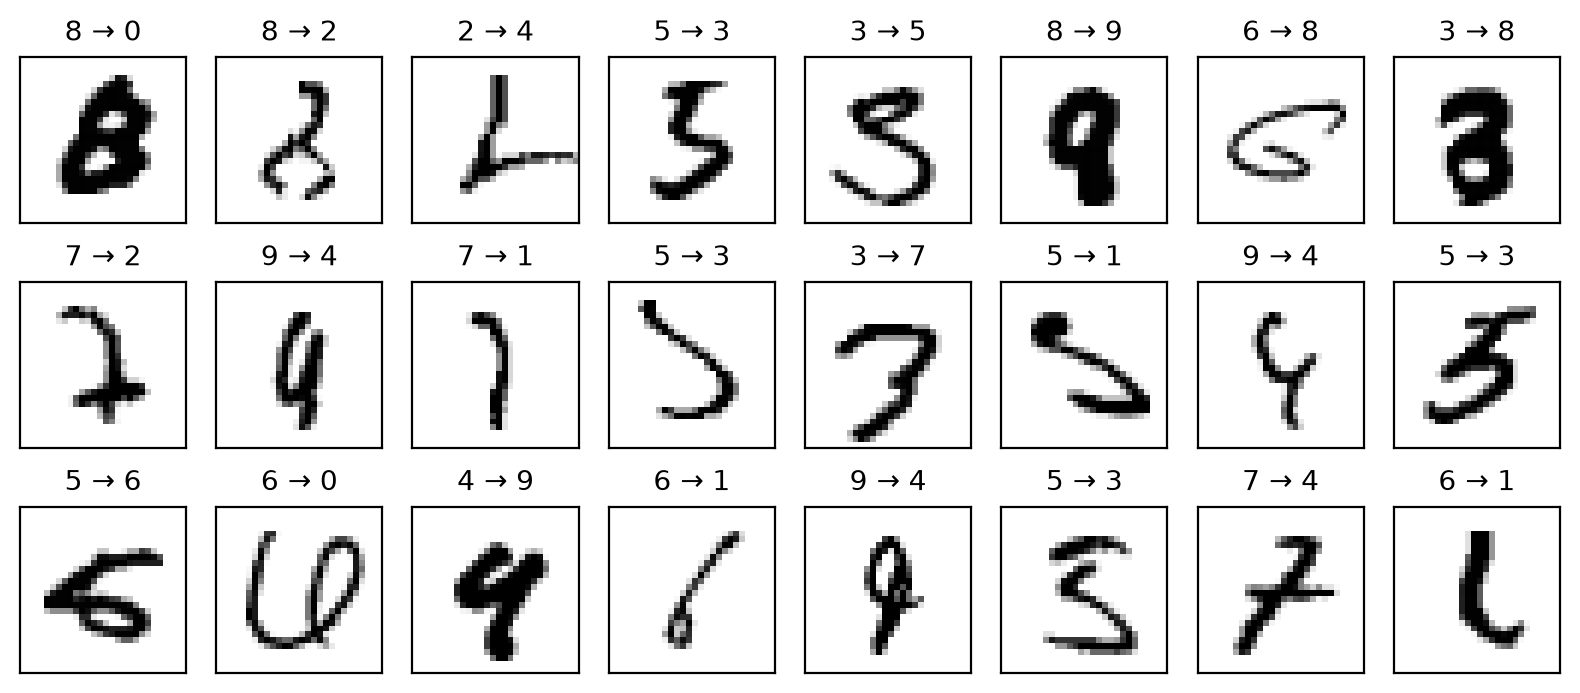
\includegraphics[width=0.85\textwidth]{figures/deep_misclassified.png}

\small DeepConvNet이 틀린 test 이미지 (처음 $24$개). ``$a\to b$''는 정답이 $a$인데 $b$로 인식했다는 뜻이다.
\end{minipage}
\end{center}

틀린 이미지 중에는 사람도 헷갈릴 만한 것이 많다. 이 정도면 남은 오류의 상당수는
\textbf{이미지 자체가 애매한 경우}이며, 정확도를 조금 더 올리기는 점점 어려워진다.

\subsection{정확도를 더 높이려면}\label{sec:higher}

MNIST에서 가장 높은 정확도를 낸 방법들도 대부분 합성곱 계층 몇 개와 완전연결 계층으로 된, 그리 깊지 않은 CNN이다.
손글씨 숫자는 비교적 단순한 문제여서 아주 깊은 network가 필요하지 않다.
정확도를 더 높이기 위해 흔히 쓰는 방법은 다음과 같다.

\begin{itemize}[leftmargin=1.5em]
\item \textbf{앙상블(ensemble):} 따로 학습한 network 여러 개의 출력(확률)을 평균한다.
각 network가 틀리는 이미지가 서로 다르면 평균이 더 정확하다.
\item \textbf{학습률 감소(learning rate decay):} 학습이 진행되면 학습률을 줄여 최솟값 근처에서 세밀하게 움직인다.
\item \textbf{데이터 확장(data augmentation):} 훈련 이미지를 조금씩 변형하여 훈련 데이터를 인위적으로 늘린다.
\end{itemize}

\paragraph{데이터 확장.}
손글씨 숫자는 조금 기울어지거나 조금 옆으로 비켜 써도 같은 숫자이다.
그러니 훈련 이미지를 \textbf{정답을 바꾸지 않을 만큼} 회전하고 이동한 이미지도 훈련 데이터로 쓸 수 있다.
\texttt{augmentation.py}의 \texttt{augment}는 미니배치의 이미지를 각각 $-10^\circ\sim10^\circ$ 사이의 무작위 각도로 회전하고,
가로와 세로로 $\pm2$픽셀 이내에서 무작위로 이동한다.

\begin{center}
\begin{minipage}{\textwidth}\centering
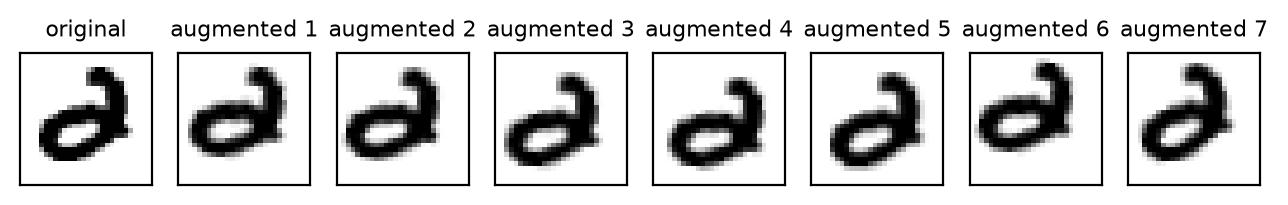
\includegraphics[width=0.9\textwidth]{figures/augment_examples.png}

\small 훈련 이미지 하나 (왼쪽)와, 그것을 무작위로 회전하고 이동한 이미지 $7$개
\end{minipage}
\end{center}

\begin{lstlisting}
    for i in range(0, len(X_train), 100):
        idx = perm[i:i + 100]
        xb, yb = X_train[idx], Y_train[idx]
        if args.augment:
            xb = augment(xb)          # a NEW random version every time
        loss = F.cross_entropy(model(xb), yb)
\end{lstlisting}

변형한 이미지를 미리 만들어 저장하지 않고, 미니배치를 꺼낼 때마다 \textbf{새로} 무작위로 변형한다.
그러면 network는 epoch마다 조금씩 다른 이미지를 보게 되어, 훈련 이미지를 외우기 어려워진다 (과대적합이 줄어든다).

\begin{center}
{\small
\begin{tabular}{@{}lcc@{}}
\toprule
훈련 데이터 & 데이터 확장 없음 & 데이터 확장 \\
\midrule
처음 $1000$장만 ($60$ epoch) & $95.38\%$ & $96.76\%$ \\
$55000$장 전부 ($20$ epoch) & $99.49\%$ & $99.50\%$ \\
\bottomrule
\end{tabular}}

DeepConvNet의 test 정확도. 같은 network, 같은 optimizer이고 훈련 이미지를 변형했는지만 다르다.
\end{center}

\begin{itemize}[leftmargin=1.5em]
\item 훈련 이미지가 $1000$장뿐이면 데이터 확장으로 정확도가 $95.38\%\to96.76\%$로 오른다.
틀린 test 이미지가 $462$개에서 $324$개로 약 $30\%$ 줄었다.
\item $55000$장을 모두 쓰면 차이가 거의 없다 ($99.49\%$ vs $99.50\%$). $0.01\%$p는 틀린 이미지 $1$개 차이로,
초깃값이나 미니배치 순서만 바꾸어도 생기는 정도이다.
훈련 데이터가 충분하면 이미 여러 기울기와 위치의 숫자를 보았기 때문이다.
\item 즉 데이터 확장은 \textbf{훈련 데이터가 부족할수록} 효과가 크다.
실제 문제에서는 데이터를 모으는 데 비용이 많이 들기 때문에 거의 항상 쓴다.
\end{itemize}

\begin{remarkbox}[정답을 바꾸지 않는 변형만 쓴다]
어떤 변형을 쓸지는 문제에 따라 다르다.
\begin{itemize}[leftmargin=1.5em]
\item 고양이 사진은 \textbf{좌우로 뒤집어도} 고양이이다. 그러나 숫자 ``$2$''나 글자 ``ㄱ''을 좌우로 뒤집으면 다른 모양이 된다.
\item 숫자 ``$6$''을 $180^\circ$ 돌리면 ``$9$''가 된다. 그래서 MNIST에서는 작은 각도만 회전한다.
\item 사진에서는 일부를 잘라 내기(crop), 크기 바꾸기, 밝기와 색 바꾸기, 잡음 더하기 등도 많이 쓴다.
\end{itemize}
데이터 확장은 ``이 정도 변형에는 답이 바뀌지 않는다''는 \textbf{사람의 지식}을 network에 알려 주는 방법이다.
\end{remarkbox}

\subsection{층을 깊게 하는 이유}\label{sec:why_deep}

층을 깊게 하는 것이 왜 좋은지 이론적으로 완전히 밝혀진 것은 아니다.
그러나 대회의 결과를 보면 상위권 network는 대부분 깊고, 다음과 같은 이점이 알려져 있다.

\paragraph{(1) 같은 수용 영역을 더 적은 매개변수로.}
입력에서 $5\times5$ 영역을 보는 출력 하나를 만드는 방법은 두 가지이다.

\begin{center}
\begin{minipage}{\textwidth}\centering
\begin{tikzpicture}[scale=0.42]
% (a) one 5x5 convolution
\begin{scope}
\fill[blue!12] (1,1) rectangle (6,6);
\draw[step=1,black!40] (0,0) grid (7,7);
\draw[blue!70!black,very thick] (1,1) rectangle (6,6);
\node[font=\scriptsize] at (3.5,-0.8) {입력};
\draw[->,thick] (7.5,3.5) -- node[above,font=\scriptsize] {$5\times5$} (10.0,3.5);
\draw[step=1,black!40] (10.5,1) grid (13.5,6);
\fill[blue!45] (11.5,3) rectangle (12.5,4);
\draw[step=1,black!40] (10.5,1) grid (13.5,6);
\node[font=\scriptsize] at (12,-0.8) {출력};
\node[font=\small] at (6.75,8.2) {(a) $5\times5$ 합성곱 한 번};
\end{scope}
% (b) two 3x3 convolutions
\begin{scope}[xshift=17cm]
\fill[blue!12] (1,1) rectangle (6,6);
\draw[step=1,black!40] (0,0) grid (7,7);
\draw[blue!70!black,very thick] (1,1) rectangle (6,6);
\node[font=\scriptsize] at (3.5,-0.8) {입력};
\draw[->,thick] (7.4,3.5) -- node[above,font=\scriptsize] {$3\times3$} (9.2,3.5);
\fill[blue!25] (10.5,2) rectangle (13.5,5);
\draw[step=1,black!40] (9.5,1) grid (14.5,6);
\draw[blue!70!black,very thick] (10.5,2) rectangle (13.5,5);
\node[font=\scriptsize] at (12,-0.8) {중간};
\draw[->,thick] (14.9,3.5) -- node[above,font=\scriptsize] {$3\times3$} (16.7,3.5);
\draw[step=1,black!40] (17.1,1) grid (20.1,6);
\fill[blue!45] (18.1,3) rectangle (19.1,4);
\draw[step=1,black!40] (17.1,1) grid (20.1,6);
\node[font=\scriptsize] at (18.6,-0.8) {출력};
\node[font=\small] at (10,8.2) {(b) $3\times3$ 합성곱 두 번};
\end{scope}
\end{tikzpicture}

\small 진한 출력 원소 하나가 의존하는 입력은 두 경우 모두 $5\times5$ 영역이다.
\end{minipage}
\end{center}

(b)에서 출력 원소 하나는 중간 데이터의 $3\times3$ 영역에 의존하고, 그 $9$개 원소는 각각 입력의 $3\times3$ 영역에 의존한다.
이 영역들을 합치면 입력의 $5\times5$ 영역이 된다 (CNN 노트 6.2절의 수용 영역, $2L+1$에서 $L=2$).
매개변수 수를 비교하면 (채널 하나, 편향 제외)

\[
\underbrace{5\times5=25}_{\text{(a)}} \qquad\text{vs}\qquad \underbrace{2\times(3\times3)=18}_{\text{(b)}},
\qquad\qquad
\underbrace{7\times7=49}_{\text{한 번}} \qquad\text{vs}\qquad \underbrace{3\times(3\times3)=27}_{\text{$3\times3$ 세 번}} .
\]

입력과 출력의 채널이 모두 $C$개이면 각각 $C^2$배가 되므로 비율은 그대로이다 ($25C^2$ vs $18C^2$).
층을 겹칠수록 차이가 커진다. 그래서 2014년 이후의 network는 큰 필터 하나보다 \textbf{작은 $3\times3$ 필터를 여러 번} 쓴다.

\paragraph{(2) 비선형성이 늘어난다.}
(b)에서는 합성곱 사이에 ReLU가 들어가므로, 같은 영역을 보면서 \textbf{비선형 함수를 한 번 더} 거친다.
활성화 함수 없이 합성곱 두 번을 하면 큰 합성곱 한 번과 같지만 (선형 함수의 합성은 선형 함수),
사이에 ReLU가 있으면 더 복잡한 함수를 표현할 수 있다.

\paragraph{(3) 문제를 계층적으로 나누어 학습한다.}
CNN 노트 6.2절에서 본 것처럼, 앞쪽 층은 에지 같은 단순한 모양에, 뒤쪽 층은 무늬, 부분, 물체에 반응한다.
``개''를 알아보는 문제를 층 하나로 풀려면 개의 모든 모습을 한 번에 배워야 한다.
층이 깊으면 앞쪽 층은 에지만, 그다음 층은 에지의 조합만 배우면 된다.
각 층이 배울 것이 \textbf{단순해지므로}, 같은 양의 데이터로 더 잘 학습할 수 있다.

\paragraph{(4) 그러나 깊을수록 학습이 어렵다.}
층을 무작정 깊게 하면 오히려 학습이 잘 되지 않는다. 2.4절의 ResNet이 이 문제를 해결한 방법이다.

% =================================================
\section{딥러닝의 초기 역사}\label{sec:history}
% =================================================

딥러닝이 크게 주목받은 계기는 2012년 이미지 인식 대회 ILSVRC에서 AlexNet이 압도적인 성적으로 우승한 일이다.
이 대회를 따라가며 대표적인 network를 살펴본다.

\subsection{이미지넷}\label{sec:imagenet}

\textbf{ImageNet}은 $1400$만 장이 넘는 이미지에 $2$만 개가 넘는 범주(class)의 이름을 붙인 데이터셋이다.
2010년부터 2017년까지 이 데이터로 \textbf{ILSVRC} (ImageNet Large Scale Visual Recognition Challenge) 대회가 열렸다.
대표 종목인 분류(classification)는 $1000$개 클래스, 훈련 이미지 약 $128$만 장이다.

\paragraph{top-5 오류.}
$1000$개 클래스 중에는 비슷한 것이 많다 (예: 개의 품종이 $100$개가 넘는다). 그래서 분류 종목은
network가 \textbf{확률이 가장 높은 $5$개 클래스}를 내고, 그 안에 정답이 없을 때만 틀린 것으로 센다.
이 비율이 \textbf{top-5 오류(top-5 error)}이다.

\begin{center}
\begin{minipage}{\textwidth}\centering
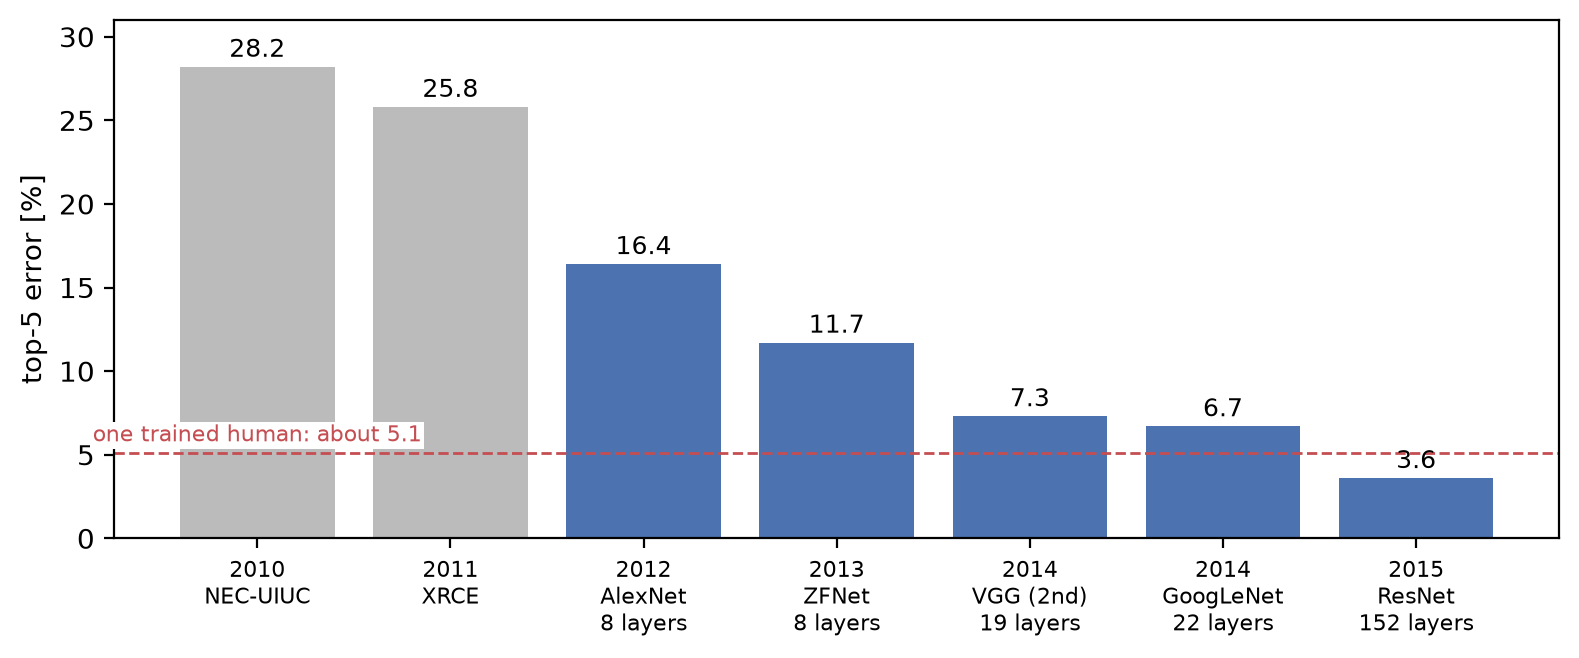
\includegraphics[width=0.9\textwidth]{figures/ilsvrc_top5.png}

\small ILSVRC 분류 종목 우승 network의 top-5 오류 (2014년은 2위였던 VGG도 함께 표시).
회색은 딥러닝이 아닌 방법이다. 사람의 오류는 한 연구자가 직접 해 본 추정치이다.
\end{minipage}
\end{center}

\begin{itemize}[leftmargin=1.5em]
\item 2011년까지는 사람이 설계한 특징 (CNN 노트 7절의 remarkbox)에 분류기를 붙인 방법이 우승하였다 (오류 $25\%$ 이상).
\item 2012년 AlexNet (CNN 노트 7.2절)이 오류를 $16.4\%$로 낮추었다. 2위와 약 $10\%$p 차이였다.
\item 그 뒤로는 모든 상위권이 딥러닝이었고, 층이 깊어지면서 오류가 계속 줄어
2015년 ResNet ($152$층)은 사람의 오류 (약 $5\%$)보다 낮은 $3.6\%$를 기록하였다.
\end{itemize}

\subsection{VGG}\label{sec:vgg}

\textbf{VGG}는 옥스퍼드 대학의 Visual Geometry Group이 만든 network (2014)로, 합성곱 계층과 풀링 계층만으로 된 \textbf{단순한 구조}가 특징이다.
가중치가 있는 계층 (합성곱 계층, 완전연결 계층)이 $16$개인 VGG16과 $19$개인 VGG19가 있다.

\begin{center}
\begin{minipage}{\textwidth}\centering
\begin{tikzpicture}[>=Latex]
% blocks: height ~ spatial size; orange bar = 2x2 max pooling
\foreach \x/\h/\w/\n/\s/\c in {0/3.2/0.35/2/224/64, 1.9/2.5/0.5/2/112/128, 3.95/1.9/0.7/3/56/256,
                               6.15/1.4/0.9/3/28/512, 8.4/1.0/0.9/3/14/512} {
  \fill[blue!14,draw=blue!60!black] (\x,{-\h/2}) rectangle ++(\w,\h);
  \fill[orange!30,draw=orange!70!black] ({\x+\w+0.12},{-\h/4}) rectangle ++(0.15,{\h/2});
  \node[font=\scriptsize,align=center,anchor=north] at ({\x+\w/2+0.1},-1.85) {conv ${\times}\n$\\$\s{\times}\s{\times}\c$};
}
\foreach \a/\b in {0.70/1.85, 2.70/3.90, 4.95/6.10, 7.35/8.35, 9.60/9.95} \draw[->] (\a,0) -- (\b,0);
\node[font=\scriptsize,align=center] at (-1.0,0) {입력\\$224{\times}224{\times}3$};
\draw[->] (-0.3,0) -- (-0.05,0);
\foreach \x/\h/\lab in {10.0/2.8/4096, 10.85/2.8/4096, 11.7/1.4/1000} {
  \fill[green!15,draw=green!45!black] (\x,{-\h/2}) rectangle ++(0.25,\h);
  \node[font=\scriptsize,anchor=north] at ({\x+0.12},-1.85) {\lab};
}
\node[font=\scriptsize] at (10.95,1.75) {완전연결};
\end{tikzpicture}

\small VGG16의 구조. 파란 블록은 $3\times3$ 합성곱 계층 $2$--$3$개 (``conv $\times2$''), 주황 막대는 $2\times2$ 최대 풀링이다.
conv 아래의 숫자는 블록의 출력 (높이$\times$너비$\times$채널 수)이다.
\end{minipage}
\end{center}

\begin{itemize}[leftmargin=1.5em]
\item 모든 합성곱은 $3\times3$, 패딩 $1$, 스트라이드 $1$이다 (1.3절의 이유). 크기를 줄이는 일은 풀링만 한다.
\item 풀링으로 크기가 반이 될 때마다 채널 수를 두 배로 늘린다 ($64\to128\to256\to512$).
DeepConvNet도 같은 규칙을 따랐다 ($16\to32\to64$).
\item 매개변수는 약 $1.38$억 개인데, 그중 첫 번째 완전연결 계층 하나가
$7\cdot7\cdot512\cdot4096+4096\approx1.03$억 개로 약 $74\%$를 차지한다.
\item 구조가 단순하고 규칙적이어서 응용하기 쉽다. 학습된 VGG를 다른 문제의 특징 추출기로 쓰는 경우가 지금도 많다 (5.1절).
\end{itemize}

\subsection{GoogLeNet}\label{sec:googlenet}

\textbf{GoogLeNet}은 구글이 만든 network로 2014년 대회에서 우승하였다 (오류 $6.7\%$, 가중치가 있는 층 $22$개).
세로 방향 (깊이)뿐 아니라 \textbf{가로 방향 (폭)}으로도 넓다는 것이 특징이다. 이 가로 방향의 구조를 \textbf{인셉션(Inception) 구조}라 한다.

\begin{center}
\begin{minipage}{\textwidth}\centering
\begin{tikzpicture}[>=Latex,
  op/.style={draw,rounded corners=2pt,minimum width=20mm,minimum height=6.5mm,font=\scriptsize,align=center},
  one/.style={op,fill=yellow!35}, big/.style={op,fill=blue!14}, pl/.style={op,fill=orange!25}]
\node[op,fill=black!6,minimum width=70mm] (prev) at (0,0) {앞 계층의 출력 ($H\times W\times C$)};
\node[one] (a1) at (-3.6,1.4) {$1\times1$ 합성곱};
\node[one] (b1) at (-1.2,1.4) {$1\times1$ 합성곱};
\node[one] (c1) at ( 1.2,1.4) {$1\times1$ 합성곱};
\node[pl]  (d1) at ( 3.6,1.4) {$3\times3$ 최대 풀링};
\node[big] (b2) at (-1.2,2.6) {$3\times3$ 합성곱};
\node[big] (c2) at ( 1.2,2.6) {$5\times5$ 합성곱};
\node[one] (d2) at ( 3.6,2.6) {$1\times1$ 합성곱};
\node[op,fill=black!6,minimum width=70mm] (cat) at (0,3.9) {채널 방향으로 이어 붙이기};
\foreach \n in {a1,b1,c1,d1} \draw[->] (prev.north -| \n) -- (\n);
\draw[->] (b1) -- (b2); \draw[->] (c1) -- (c2); \draw[->] (d1) -- (d2);
\draw[->] (a1) -- (cat.south -| a1);
\foreach \n in {b2,c2,d2} \draw[->] (\n) -- (cat.south -| \n);
\end{tikzpicture}

\small 인셉션 구조. 크기가 다른 필터와 풀링을 나란히 적용하고, 결과를 채널 방향으로 이어 붙인다.
노란 상자가 $1\times1$ 합성곱이다.
\end{minipage}
\end{center}

크기가 다른 필터 ($1\times1$, $3\times3$, $5\times5$)를 \textbf{동시에} 쓰므로,
작은 무늬와 큰 무늬를 함께 볼 수 있다. 어떤 크기가 중요한지는 network가 학습으로 정한다.
모든 경로의 공간 크기가 같도록 패딩을 주고, 출력은 채널 방향으로 이어 붙인다.

\paragraph{$1\times1$ 합성곱.}
$1\times1$ 필터는 공간 방향으로는 한 픽셀만 보지만, \textbf{채널 방향으로는 모든 채널}을 본다.
위치 $(i,j)$의 출력 채널 $k$는
\[
y_{k,i,j}=\sum_{c=1}^{C} w_{k,c}\,x_{c,i,j}+b_k ,
\]
즉 \textbf{픽셀마다 같은 Affine 계층} ($C$개 입력 $\to$ $FN$개 출력)을 적용하는 것이다.
출력 채널 수 $FN$을 $C$보다 작게 하면 공간 크기는 그대로 두고 \textbf{채널 수만 줄인다}.
인셉션 구조는 큰 합성곱 앞에 $1\times1$ 합성곱을 두어 계산량과 매개변수를 크게 줄인다.

\begin{thinkbox}[예: $1\times1$ 합성곱으로 줄이기]
입력이 $256$채널이고 $5\times5$ 필터 $64$개를 적용한다고 하자 (편향 제외).
\begin{itemize}[leftmargin=1.5em]
\item 바로 적용: $5\cdot5\cdot256\cdot64=409600$개.
\item $1\times1$ 합성곱으로 먼저 $32$채널로 줄인 뒤 적용: $1\cdot1\cdot256\cdot32+5\cdot5\cdot32\cdot64=8192+51200=59392$개.
\end{itemize}
매개변수가 약 $\frac{1}{7}$이 된다. 출력의 원소 하나를 계산하는 곱셈 수도 같은 비율로 줄어든다.
GoogLeNet 전체의 매개변수는 약 $700$만 개로 AlexNet (약 $6000$만 개)의 약 $\frac{1}{10}$이다.
\end{thinkbox}

\subsection{ResNet}\label{sec:resnet}

\textbf{ResNet} (Residual Network)은 마이크로소프트 연구팀이 만든 network로 2015년 대회에서 우승하였다 ($152$층, 오류 $3.6\%$).

\paragraph{깊게 하면 오히려 나빠진다.}
층을 깊게 하는 것이 좋다고 해서 무작정 쌓으면, 어느 정도부터는 \textbf{훈련 데이터에서조차} 성능이 나빠진다.
과대적합(훈련은 잘 되는데 test가 나쁨)과는 다른 문제로, 깊은 network의 \textbf{최적화 자체가 어려워지는} 것이다.
간단한 실험을 해 보자 (\texttt{resnet\_skip.py}).
MNIST 이미지를 길이 $784$의 벡터로 펼쳐 넣고, ``Affine $\to$ ReLU $\to$ Affine $\to$ ReLU''를 블록 하나로 하여
블록 $3$개 ($8$층)인 network와 블록 $30$개 ($62$층)인 network를 같은 방법 (He 초깃값, Adam, 학습률 $0.001$)으로 학습시킨다.

\begin{center}
\begin{minipage}{\textwidth}\centering
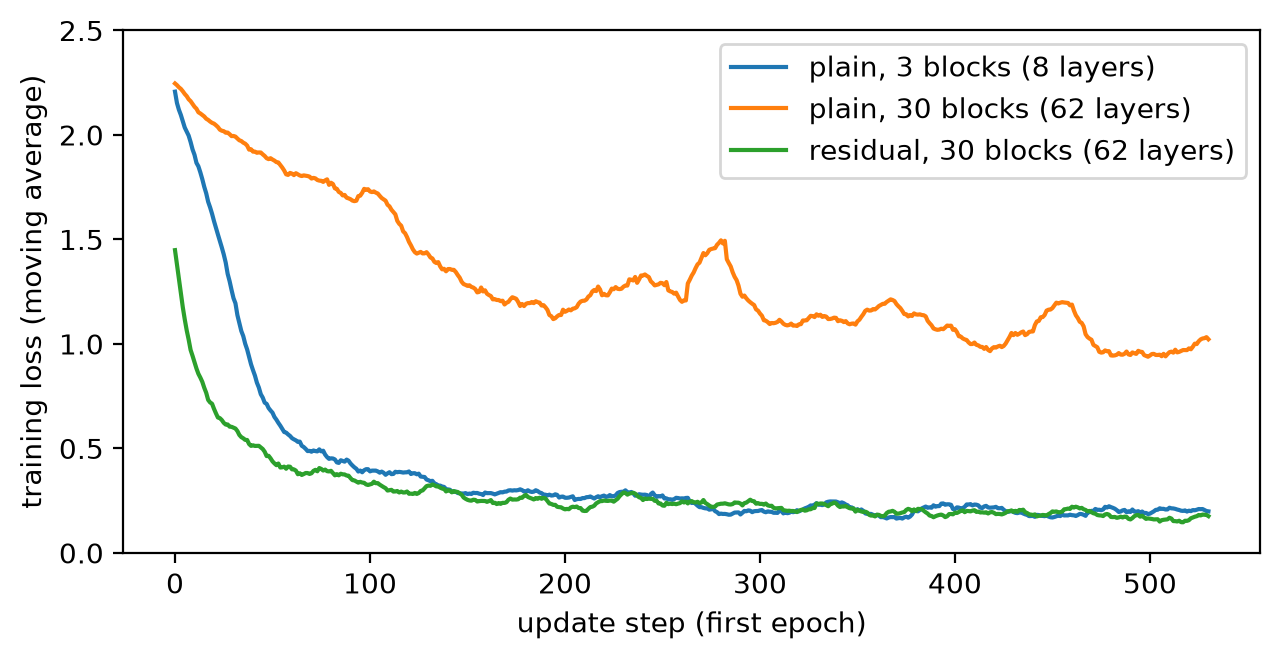
\includegraphics[width=0.72\textwidth]{figures/resnet_loss.png}

\small 첫 epoch의 훈련 손실 (최근 $20$번 갱신의 평균). 층마다 폭은 $64$이다.
\end{minipage}
\end{center}

$62$층 일반 network (주황)는 $8$층 network (파랑)보다 표현력이 훨씬 큰데도, 훈련 손실이 $1$ 근처에서 잘 내려가지 않는다.
같은 $62$층에 \textbf{skip connection}만 추가한 network (초록)는 $8$층 network만큼, 처음에는 그보다 더 빨리 학습된다.

\paragraph{스킵 연결 (skip connection).}
ResNet의 블록은 입력 $x$를 몇 개의 층에 통과시킨 결과 $F(x)$에 \textbf{입력 $x$를 그대로 더한다}.

\begin{center}
\begin{minipage}{\textwidth}\centering
\begin{tikzpicture}[>=Latex,
  lay/.style={draw,rounded corners=2pt,minimum width=26mm,minimum height=6.5mm,font=\small,fill=blue!12}]
\node (x) at (0,0) {$x$};
\node[lay] (w1) at (0,-1.1) {가중치 층};
\node[lay] (w2) at (0,-2.5) {가중치 층};
\node[draw,circle,inner sep=1pt] (plus) at (0,-3.6) {$+$};
\node (y) at (0,-4.6) {$F(x)+x$};
\draw[->] (x) -- (w1);
\draw[->] (w1) -- node[right,font=\scriptsize] {ReLU} (w2);
\draw[->] (w2) -- (plus);
\draw[->] (plus) -- node[right,font=\scriptsize] {ReLU} (y);
\draw[->,thick,deepblue] (x.east) -- ++(2.2,0) |- node[pos=0.25,right,font=\small] {$x$ (그대로)} (plus.east);
\draw[decorate,decoration={brace,amplitude=4pt}] (-1.55,-2.85) -- (-1.55,-0.75) node[midway,left=4pt] {$F(x)$};
\end{tikzpicture}

\small ResNet의 블록. 오른쪽의 길이 skip connection (shortcut, identity mapping)이다.
\end{minipage}
\end{center}

코드로는 한 줄 차이이다 (\texttt{resnet\_skip.py}).

\begin{lstlisting}
        for l1, l2 in self.blocks:
            f = l2(F.relu(l1(h)))
            h = F.relu(h + f) if self.skip else F.relu(f)
\end{lstlisting}

\paragraph{왜 학습이 쉬워지는가?}
\begin{itemize}[leftmargin=1.5em]
\item \textbf{역전파:} $y=x+F(x)$이면 연쇄법칙에 의해
\[
\pd{L}{x}=\pd{L}{y}\,\Bigl(1+\pd{F}{x}\Bigr)=\pd{L}{y}+\pd{L}{y}\pd{F}{x} .
\]
덧셈 노드는 기울기를 그대로 나누어 주므로 (역전파 노트), 위층의 기울기 $\pd{L}{y}$가 \textbf{줄어들지 않고 그대로} 아래층에 전달된다.
일반 network에서는 기울기가 층마다 $\pd{F}{x}$와 곱해지므로, 층이 많으면 매우 작아지거나 커지기 쉽다.
(스칼라로 생각하면 $30$층을 지날 때 일반 network는 $\prod_l f_l'$, ResNet은 $\prod_l(1+f_l')$이다.)
\item \textbf{잔차(residual)를 학습한다:} 블록이 만들어야 하는 함수가 $H(x)$라면, 블록은 $F(x)=H(x)-x$만 학습하면 된다.
특히 어떤 블록이 필요 없으면 $F(x)=0$, 즉 가중치를 $0$ 근처로 두기만 하면 된다.
그래서 층을 더해도 적어도 나빠지지는 않는다. 이름의 residual은 이 $H(x)-x$를 뜻한다.
\end{itemize}

ResNet은 이 블록을 합성곱 계층으로 만들어 $150$층 이상 쌓았다 (블록 안의 합성곱은 VGG처럼 $3\times3$).
skip connection은 지금도 거의 모든 깊은 network에 쓰인다.
요즘 언어 모델의 기반인 \textbf{Transformer}도 블록마다 $x+F(x)$ 형태의 연결을 쓴다.

\begin{remarkbox}[전이 학습 (transfer learning)]
ImageNet으로 학습한 VGG나 ResNet의 가중치는 공개되어 있다.
이 가중치를 \textbf{초깃값}으로 하여, 우리가 가진 (보통 훨씬 작은) 데이터셋으로 다시 학습하는 것을 \textbf{전이 학습}이라 한다.
앞쪽 층이 배운 에지와 무늬는 대부분의 사진에 공통이므로, 마지막 완전연결 계층만 새 클래스 수에 맞게 바꾸어 학습해도
처음부터 학습하는 것보다 훨씬 적은 데이터로 좋은 성능을 얻는 경우가 많다.
PyTorch에서는 (torchvision 패키지를 설치한 뒤) 다음과 같이 한다.
\begin{lstlisting}[numbers=none]
from torchvision.models import resnet18, ResNet18_Weights
model = resnet18(weights=ResNet18_Weights.DEFAULT)     # trained on ImageNet
model.fc = nn.Linear(model.fc.in_features, 5)          # new last layer: 5 classes
\end{lstlisting}
\end{remarkbox}

% =================================================
\section{더 빠르게}\label{sec:faster}
% =================================================

빅데이터와 깊은 network를 학습하려면 엄청난 계산이 필요하다.
1.1절에서 본 것처럼 numpy로는 MNIST조차 몇 시간이 걸린다. 어떻게 빠르게 할 수 있을까?

\subsection{시간은 어디에 쓰이는가}\label{sec:where_time}

\texttt{speed\_precision.py}는 numpy의 DeepConvNet으로 미니배치 $100$개의 순전파와 역전파를 하면서 계층마다 걸린 시간을 잰다.

\begin{center}
\begin{minipage}{\textwidth}\centering
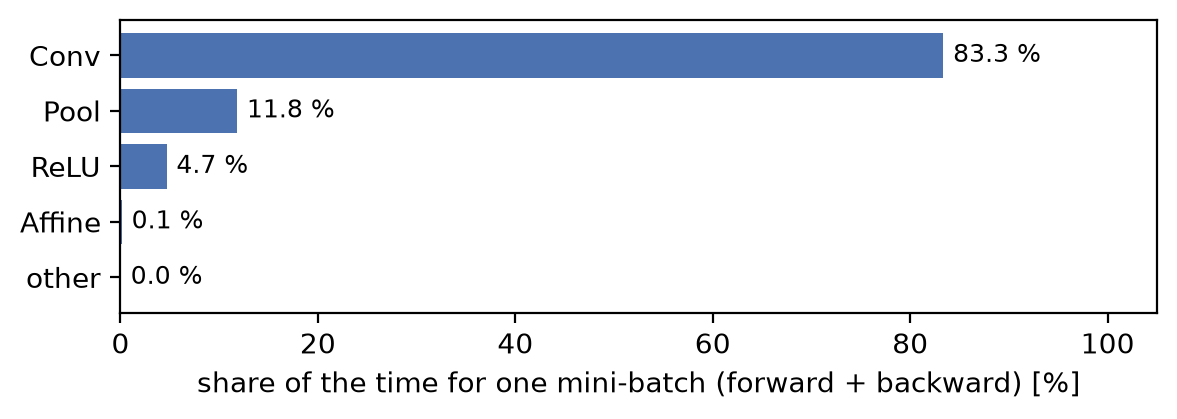
\includegraphics[width=0.62\textwidth]{figures/time_by_layer.png}

\small DeepConvNet (numpy)의 미니배치 하나 (순전파 + 역전파)에서 계층 종류별로 걸린 시간의 비율
\end{minipage}
\end{center}

시간의 약 83\%가 \textbf{합성곱 계층}에 쓰인다.
더 큰 network에서도 마찬가지여서, AlexNet에서는 순전파 시간의 약 $95\%$ (GPU)와 약 $89\%$ (CPU)가 합성곱 계층이었다는 측정이 있다.
그러므로 딥러닝을 빠르게 하는 것은 곧 \textbf{합성곱을 빠르게} 하는 것이다.
그리고 im2col (CNN 노트 4절)을 쓰면 합성곱은 하나의 큰 \textbf{행렬곱}이다.
결국 핵심은 \textbf{대량의 곱셈-덧셈 (행렬곱)을 빠르게} 하는 것이다.

\subsection{GPU를 활용한 고속화}\label{sec:gpu}

\textbf{GPU} (Graphics Processing Unit)는 원래 화면의 수많은 픽셀을 동시에 계산하는 그래픽 전용 장치였다.
CPU는 복잡한 일을 하는 코어가 수 개에서 수십 개 있고, GPU는 단순한 곱셈-덧셈을 하는 코어가 \textbf{수천 개} 있다.

행렬곱 $C=AB$의 원소 $c_{ij}=\sum_k a_{ik}b_{kj}$는 \textbf{서로 독립}이다. $c_{11}$을 계산하는 데 $c_{12}$가 필요 없다.
그래서 수천 개의 코어에 나누어 동시에 계산할 수 있다. 딥러닝은 GPU가 잘하는 일 그 자체이다.
2012년 AlexNet도 GPU $2$개로 학습하였고, 수십 일 걸리던 학습이 며칠로 줄어든 것이 딥러닝 발전의 큰 원동력이었다.
현재 딥러닝용 GPU는 주로 NVIDIA 제품이며, CUDA라는 GPU 프로그래밍 환경과 그 위의 딥러닝용 라이브러리 (cuDNN)를 쓴다.

\paragraph{numpy와 PyTorch.}
같은 CPU에서도 라이브러리에 따라 속도가 크게 다르다. DeepConvNet의 미니배치 하나 (순전파 + 역전파)를 비교하면

\begin{center}
{\small
\begin{tabular}{@{}lr@{}}
\toprule
구현 & 미니배치 $100$개, 순전파 + 역전파 \\
\midrule
numpy (\texttt{deep\_convnet.py}) & 약 626 ms \\
PyTorch, CPU & 약 46 ms \\
\bottomrule
\end{tabular}}
\end{center}

PyTorch는 im2col처럼 큰 임시 배열을 만들지 않고, 합성곱 전용으로 최적화된 C++ 코드로 CPU 코어 여러 개를 함께 쓴다.
GPU가 있으면 코드 한 줄로 GPU에서 계산한다.

\begin{lstlisting}[numbers=none]
device = "cuda" if torch.cuda.is_available() else "cpu"
model = model.to(device)                 # the parameters go to the GPU
xb, yb = xb.to(device), yb.to(device)    # and every mini-batch too
\end{lstlisting}

\subsection{분산 학습}\label{sec:distributed}

GPU 하나로도 오래 걸리면 여러 GPU, 여러 컴퓨터로 나누어 계산한다. 가장 많이 쓰는 방법은 \textbf{데이터 병렬 (data parallel)}이다.

\begin{center}
\begin{minipage}{\textwidth}\centering
\begin{tikzpicture}[>=Latex,
  gpu/.style={draw,rounded corners=2pt,fill=blue!10,minimum width=24mm,minimum height=9mm,font=\scriptsize,align=center}]
\node[draw,rounded corners=2pt,fill=black!5,minimum width=40mm,minimum height=7mm,font=\scriptsize] (mb) at (0,0) {미니배치 $400$개};
\foreach \k/\x in {1/-4.5,2/-1.5,3/1.5,4/4.5} {
  \node[gpu] (g\k) at (\x,-1.7) {GPU \k\\(같은 매개변수 $W$)};
  \draw[->] (mb.south) -- node[left,font=\tiny,pos=0.7] {$100$개} (g\k.north);
  \node[font=\scriptsize] (d\k) at (\x,-2.75) {$\grad L_\k$};
  \draw[->] (g\k) -- (d\k);
}
\node[draw,rounded corners=2pt,fill=green!12,minimum width=60mm,minimum height=7mm,font=\scriptsize] (avg) at (0,-3.9)
  {평균 $\grad L=\frac14(\grad L_1+\grad L_2+\grad L_3+\grad L_4)$ $\;\to\;$ $W\leftarrow W-\eta\,\grad L$};
\foreach \k in {1,...,4} \draw[->] (d\k) -- (avg.north -| d\k);
\end{tikzpicture}

\small 데이터 병렬. GPU마다 미니배치의 일부로 기울기를 구하고, 평균한 기울기로 모든 GPU의 매개변수를 똑같이 갱신한다.
\end{minipage}
\end{center}

손실이 미니배치의 평균 $L=\frac1B\sum_{n=1}^{B}\ell_n$이므로, 미니배치를 크기가 같은 $K$개로 나누어
$L_k=\frac{K}{B}\sum_{n\in\text{조각 }k}\ell_n$이라 하면
\[
\grad L=\frac1B\sum_{n=1}^{B}\grad\ell_n=\frac1K\sum_{k=1}^{K}\grad L_k .
\]
즉 GPU $K$개가 나누어 구한 기울기를 평균하면 \textbf{GPU 하나로 구한 기울기와 정확히 같다}.
다만 GPU 사이에 기울기를 주고받는 통신 시간이 들어서, GPU를 $100$개 쓴다고 $100$배 빨라지지는 않는다.
network가 너무 커서 GPU 하나의 메모리에 들어가지 않으면 \textbf{계층을 나누어} 여러 GPU에 두는 모델 병렬(model parallel)도 쓴다.
요즘의 큰 언어 모델은 수천 개 이상의 GPU에서 두 방법을 함께 써서 학습한다.

\subsection{연산 정밀도와 비트 줄이기}\label{sec:precision}

numpy는 기본으로 \textbf{64비트} 부동소수점수 (\texttt{float64}, 배정밀도)를 쓴다.
그런데 신경망은 원래 잡음에 강하다 (드롭아웃은 일부러 노드를 지우는데도 잘 학습된다).
숫자 하나를 더 적은 비트로 나타내면 메모리가 줄고, 같은 시간에 더 많이 계산하고 더 많이 주고받을 수 있다.

\begin{center}
{\small
\begin{tabular}{@{}lccccl@{}}
\toprule
형식 & 비트 & 지수 & 가수 & 가장 큰 수 & $1$ 다음의 수 \\
\midrule
\texttt{float64} (배정밀도) & $64$ & $11$ & $52$ & $\approx1.8\times10^{308}$ & $1+2^{-52}$ \\
\texttt{float32} (단정밀도) & $32$ & $8$ & $23$ & $\approx3.4\times10^{38}$ & $1+2^{-23}$ \\
\texttt{float16} (반정밀도) & $16$ & $5$ & $10$ & $65504$ & $1+2^{-10}\approx1.001$ \\
\texttt{bfloat16} & $16$ & $8$ & $7$ & $\approx3.4\times10^{38}$ & $1+2^{-7}\approx1.008$ \\
\bottomrule
\end{tabular}}
\end{center}

\texttt{float16}은 십진수로 약 $3$자리의 정밀도뿐이다. 예를 들어
\[
\texttt{np.float16(1) + np.float16(0.0001)} = 1, \qquad \texttt{np.float16(70000)} = \texttt{inf} .
\]
이렇게 거친 수로 계산해도 괜찮을까?
1.1절에서 학습한 DeepConvNet의 매개변수와 입력을 \texttt{float16}으로 바꾸어 test 이미지 $2000$장을 인식해 보자 (\texttt{speed\_precision.py}).

\begin{center}
{\small
\begin{tabular}{@{}lccr@{}}
\toprule
형식 & 매개변수 메모리 & test 정확도 (처음 $2000$장) \\
\midrule
\texttt{float64} & $965$ KB & $99.25\%$ \\
\texttt{float32} & $483$ KB & $99.25\%$ \\
\texttt{float16} & $241$ KB & $99.25\%$ \\
\bottomrule
\end{tabular}}
\end{center}

세 경우의 정확도가 같을 뿐 아니라, $2000$장 각각의 예측이 \textbf{하나도 다르지 않았다}.
출력 점수는 최대 $0.03$ 정도 달라졌지만 (점수의 크기는 최대 약 $80$), 가장 큰 점수의 클래스는 바뀌지 않았다.
매개변수의 메모리는 절반, 다시 절반으로 줄었다.
(numpy는 \texttt{float16} 계산을 빠르게 하지 못하므로 이 실험에서 시간은 줄지 않는다.
16비트 계산은 GPU 등 그것을 지원하는 하드웨어에서 빨라진다.)
\begin{itemize}[leftmargin=1.5em]
\item 딥러닝에서는 \textbf{\texttt{float32}가 기본}이다 (PyTorch의 기본값).
\item 학습에도 \texttt{float16}이나 \texttt{bfloat16}을 섞어 쓰는 \textbf{혼합 정밀도 학습}(mixed precision)이 흔하다.
기울기처럼 아주 작아질 수 있는 값은 \texttt{float32}로 보관하고, 큰 행렬곱만 16비트로 계산한다.
\texttt{bfloat16}은 가수를 줄이는 대신 지수를 \texttt{float32}만큼 두어, 아주 크거나 작은 수도 넘치지 않게 한 형식이다.
\item 학습이 끝난 network를 휴대폰 등에서 쓸 때는 \textbf{8비트 정수}(int8)나 그보다 적은 비트로 바꾸는 \textbf{양자화}(quantization)도 쓴다.
\end{itemize}

% =================================================
\section{딥러닝의 활용}\label{sec:applications}
% =================================================

지금까지는 이미지 전체에 클래스 하나를 붙이는 \textbf{분류} 문제를 보았다.
CNN이 뽑은 특징은 다른 많은 문제에도 쓰인다.

\subsection{사물 검출}\label{sec:detection}

\textbf{사물 검출(object detection)}은 이미지 속 물체 \textbf{각각의 위치 (사각형, bounding box)와 클래스}를 찾는 문제이다.
물체가 몇 개인지 미리 모르고, 크기와 위치도 다양하므로 분류보다 어렵다.

\begin{center}
\begin{minipage}{\textwidth}\centering
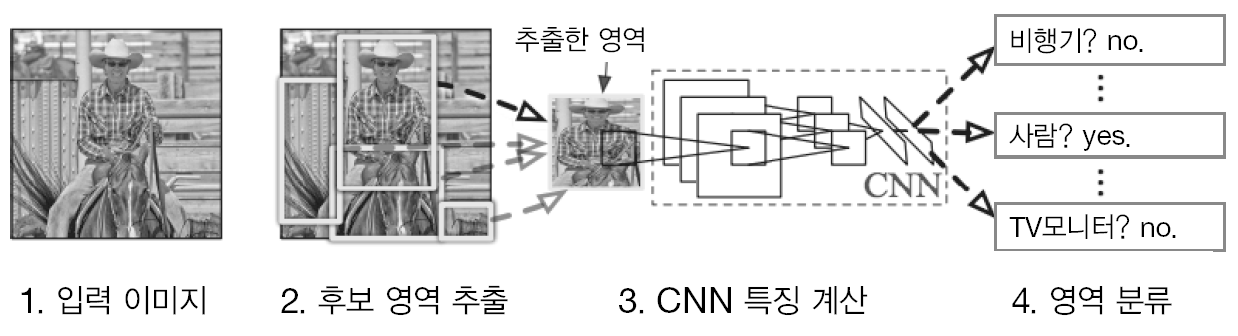
\includegraphics[width=0.9\textwidth]{figures/rcnn.png}

\small R-CNN의 처리 흐름 (Girshick 등, 2014)
\end{minipage}
\end{center}

\textbf{R-CNN} (Regions with CNN features)은 다음 순서로 검출한다.
\begin{enumerate}[leftmargin=1.8em]
\item 물체가 있을 만한 영역의 후보를 약 $2000$개 뽑는다 (CNN이 아닌, 색과 질감이 비슷한 영역을 묶는 방법).
\item 후보 영역 각각을 같은 크기로 바꾸어 CNN에 넣고 특징을 계산한다.
\item 특징으로 영역을 분류한다 (``비행기? 아니다'', ``사람? 그렇다'', $\ldots$).
\end{enumerate}
후보마다 CNN을 따로 계산하므로 매우 느렸다. 그 뒤 이미지 전체에 CNN을 한 번만 계산하는 Fast R-CNN,
후보 영역까지 CNN으로 뽑는 Faster R-CNN (2015),
이미지를 격자로 나누어 한 번에 위치와 클래스를 모두 출력하는 \textbf{YOLO} (You Only Look Once, 2016) 등이 나와,
지금은 동영상에서 실시간으로 검출할 수 있다.

\paragraph{예측이 맞았는지 어떻게 재는가: IoU.}
예측한 사각형 $A$와 정답 사각형 $B$가 얼마나 겹치는지는
\[
\text{IoU}=\frac{\text{넓이}(A\cap B)}{\text{넓이}(A\cup B)}
\]
(Intersection over Union)로 잰다. 완전히 겹치면 $1$, 전혀 안 겹치면 $0$이다. 보통 $\text{IoU}\ge0.5$이면 맞은 것으로 센다.

\begin{center}
\begin{minipage}{\textwidth}\centering
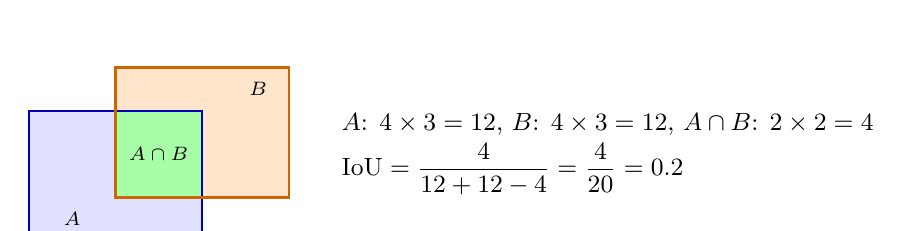
\begin{tikzpicture}[scale=0.55]
\fill[blue!12] (0,0) rectangle (4,3);
\fill[orange!20] (2,1) rectangle (6,4);
\fill[green!35] (2,1) rectangle (4,3);
\draw[blue!70!black,thick] (0,0) rectangle (4,3);
\draw[orange!80!black,thick] (2,1) rectangle (6,4);
\node[font=\scriptsize] at (1,0.5) {$A$};
\node[font=\scriptsize] at (5.3,3.5) {$B$};
\node[font=\scriptsize] at (3,2) {$A\cap B$};
\node[font=\small,right,align=left] at (7,2) {$A$: $4\times3=12$, $B$: $4\times3=12$, $A\cap B$: $2\times2=4$\\[2pt]
$\text{IoU}=\dfrac{4}{12+12-4}=\dfrac{4}{20}=0.2$};
\end{tikzpicture}
\end{minipage}
\end{center}

\subsection{분할}\label{sec:segmentation}

\textbf{분할(segmentation)}은 이미지를 \textbf{픽셀 단위로} 분류하는 문제이다.
모든 픽셀에 ``사람'', ``오토바이'', ``배경'' 같은 클래스를 붙인다.

\begin{center}
\begin{minipage}{\textwidth}\centering
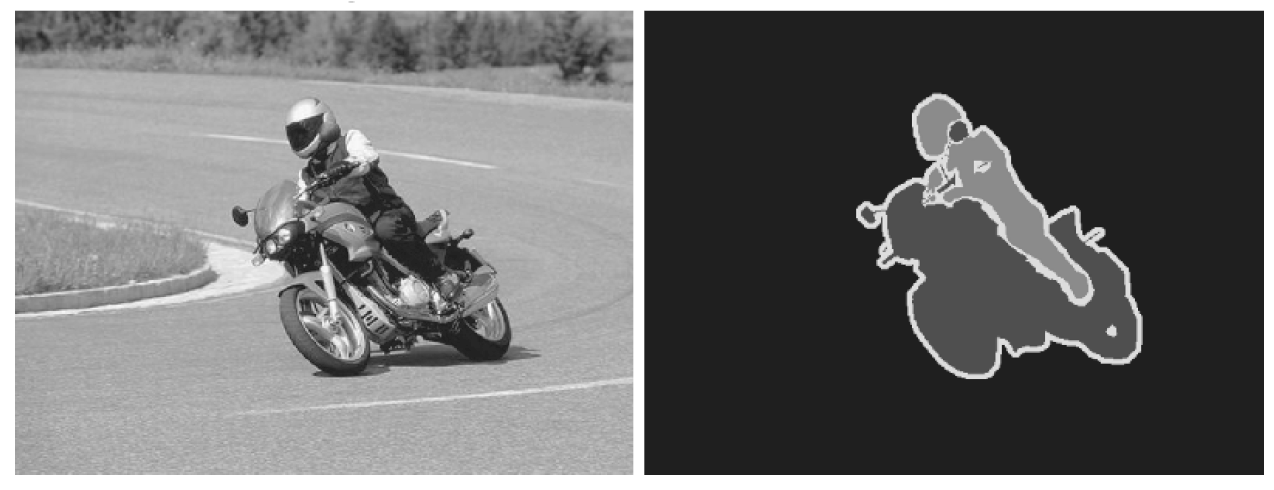
\includegraphics[width=0.7\textwidth]{figures/segmentation.png}

\small 분할의 예. 왼쪽이 입력, 오른쪽이 픽셀마다 클래스를 칠한 결과이다.
\end{minipage}
\end{center}

가장 단순한 방법은 픽셀마다 그 주변을 잘라 분류하는 것이지만, 픽셀 수만큼 순전파를 해야 하므로 너무 느리다.
\textbf{FCN} (Fully Convolutional Network, 2015)은 network 전체를 \textbf{합성곱 계층만으로} 만들어 한 번의 순전파로 모든 픽셀을 분류한다.

\begin{center}
\begin{minipage}{\textwidth}\centering
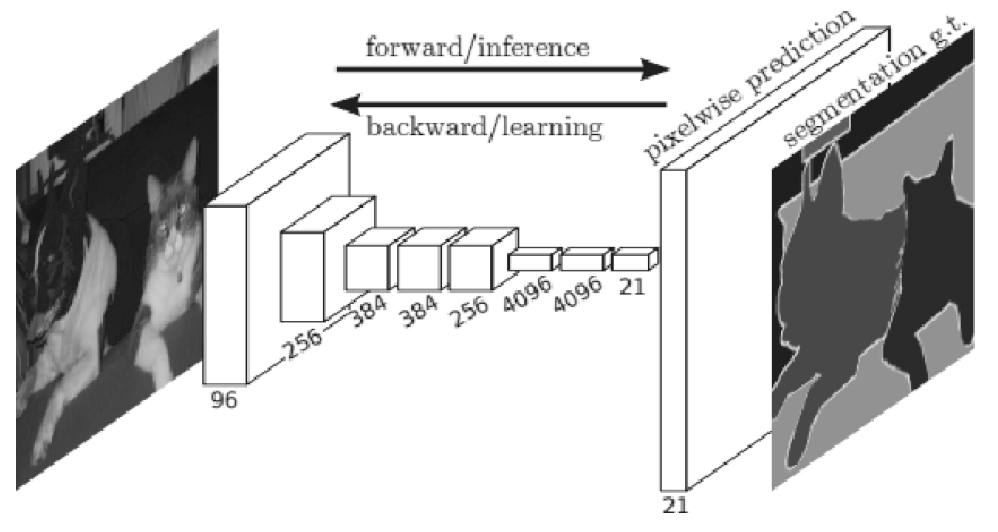
\includegraphics[width=0.7\textwidth]{figures/fcn.png}

\small FCN의 구조 (Long 등, 2015). 마지막 출력은 클래스 수 ($21$)만큼의 채널을 가진 입력 크기의 이미지이다.
\end{minipage}
\end{center}

\begin{itemize}[leftmargin=1.5em]
\item \textbf{완전연결 계층을 합성곱 계층으로:} $7\times7\times512$ 입력에 대한 완전연결 계층 ($4096$개 출력)은
$7\times7$ 필터 $4096$개의 합성곱과 같은 계산이다 (CNN 노트에서 본 LeNet의 C5와 같다).
합성곱이므로 입력이 더 크면 출력도 $1\times1$이 아니라 공간 크기를 가진 맵이 된다.
\item \textbf{크기 되돌리기:} 풀링으로 작아진 맵을 입력 크기로 다시 키운다 (upsampling).
간단히는 쌍선형 보간 (bilinear interpolation)을 쓰고, 학습할 수 있는 \textbf{전치 합성곱} (transposed convolution)도 쓴다.
\end{itemize}

\subsection{사진 캡션 생성}\label{sec:caption}

사진을 보고 그 내용을 설명하는 문장을 만드는 연구도 있다.

\begin{center}
\begin{minipage}{\textwidth}\centering
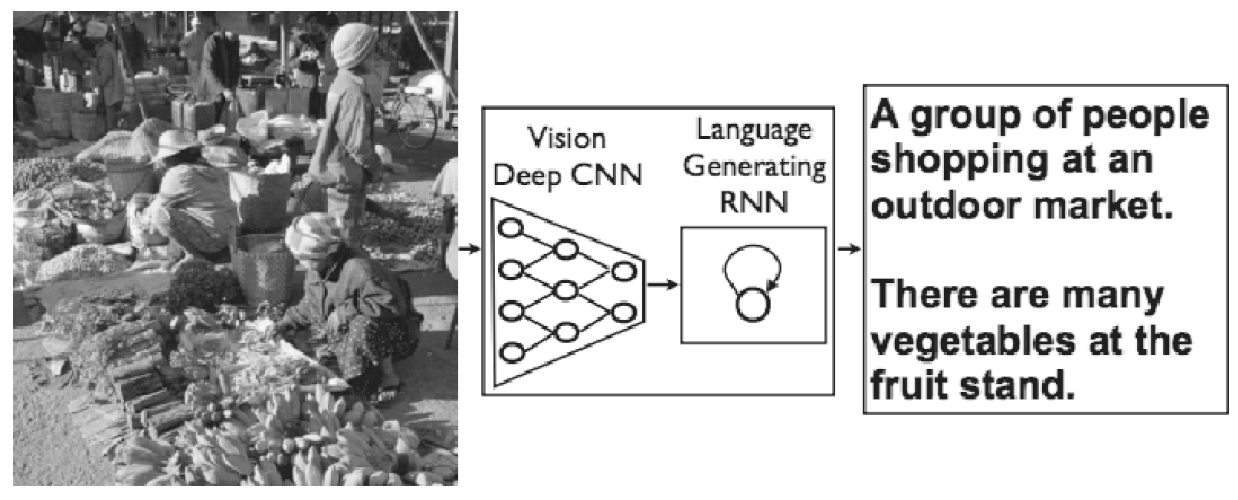
\includegraphics[width=0.75\textwidth]{figures/caption_nic.png}

\small NIC의 구조 (Vinyals 등, 2015): CNN이 사진을 벡터로 요약하고, RNN이 그 벡터로부터 단어를 하나씩 만든다.
\end{minipage}
\end{center}

\textbf{NIC} (Neural Image Caption)는 깊은 CNN과 자연어를 다루는 \textbf{RNN} (Recurrent Neural Network, 순환 신경망)으로 되어 있다.
CNN이 사진의 특징을 뽑으면, 그 특징을 RNN의 처음 입력으로 하여 RNN이 앞에서 만든 단어들을 보고 다음 단어를 하나씩 만든다.
사진과 문장처럼 여러 종류의 정보를 함께 다루는 것을 \textbf{멀티모달(multimodal)} 처리라 한다.
지금은 RNN 대신 Transformer를 쓰며, 사진에 대해 질문하고 답하는 모델로 발전하였다.

% =================================================
\section{딥러닝의 미래}\label{sec:future}
% =================================================

여기서는 2015--2016년 무렵 ``딥러닝으로 이런 것도 된다''며 주목받은 예를 본다.
지금은 대부분 실제로 쓰이는 기술이 되었다.

\subsection{이미지 스타일 변환}\label{sec:style}

\begin{center}
\begin{minipage}{\textwidth}\centering
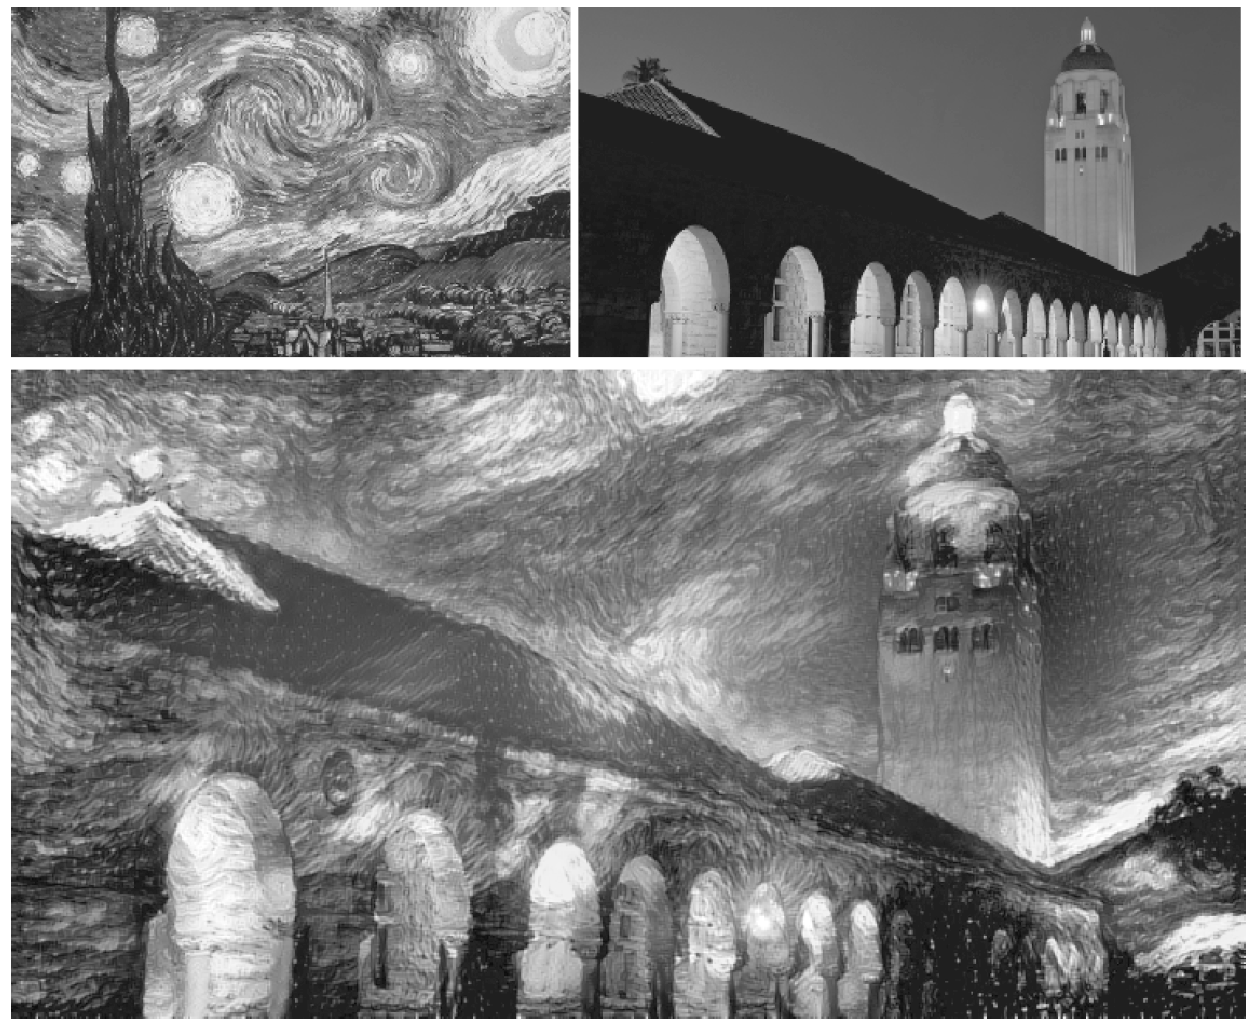
\includegraphics[width=0.6\textwidth]{figures/style_transfer.png}

\small 스타일 변환 (Gatys 등, 2015). 왼쪽 위 그림의 화풍을 오른쪽 위 사진에 입힌 결과가 아래이다.
\end{minipage}
\end{center}

학습된 CNN (VGG)을 그대로 두고, \textbf{이미지의 픽셀}을 변수로 하여 다음 손실을 줄이도록 경사하강법을 쓴다.
\begin{itemize}[leftmargin=1.5em]
\item \textbf{내용 손실:} 만드는 이미지와 사진의 \textbf{뒤쪽 층 특징 맵}이 비슷해지게 한다. 뒤쪽 층은 물체의 배치와 모양을 담고 있다.
\item \textbf{스타일 손실:} 만드는 이미지와 그림의 \textbf{그람 행렬}이 비슷해지게 한다.
층의 특징 맵을 채널마다 길이 $HW$인 벡터 $\vect f_1,\ldots,\vect f_C$로 펼쳤을 때 $G_{ij}=\vect f_i\cdot\vect f_j$이다.
``어떤 무늬 필터들이 함께 반응하는가''를 위치와 상관없이 요약한 것이어서, 붓 터치나 색감 같은 화풍을 나타낸다.
\end{itemize}
매개변수가 아니라 \textbf{입력}에 대한 기울기를 쓴다는 점이 새롭지만, 계산은 지금까지 한 역전파와 같다.
(역전파는 원래 입력 쪽 기울기 \texttt{dX}까지 계산한다.)

\subsection{이미지 생성}\label{sec:generation}

\begin{center}
\begin{minipage}{\textwidth}\centering
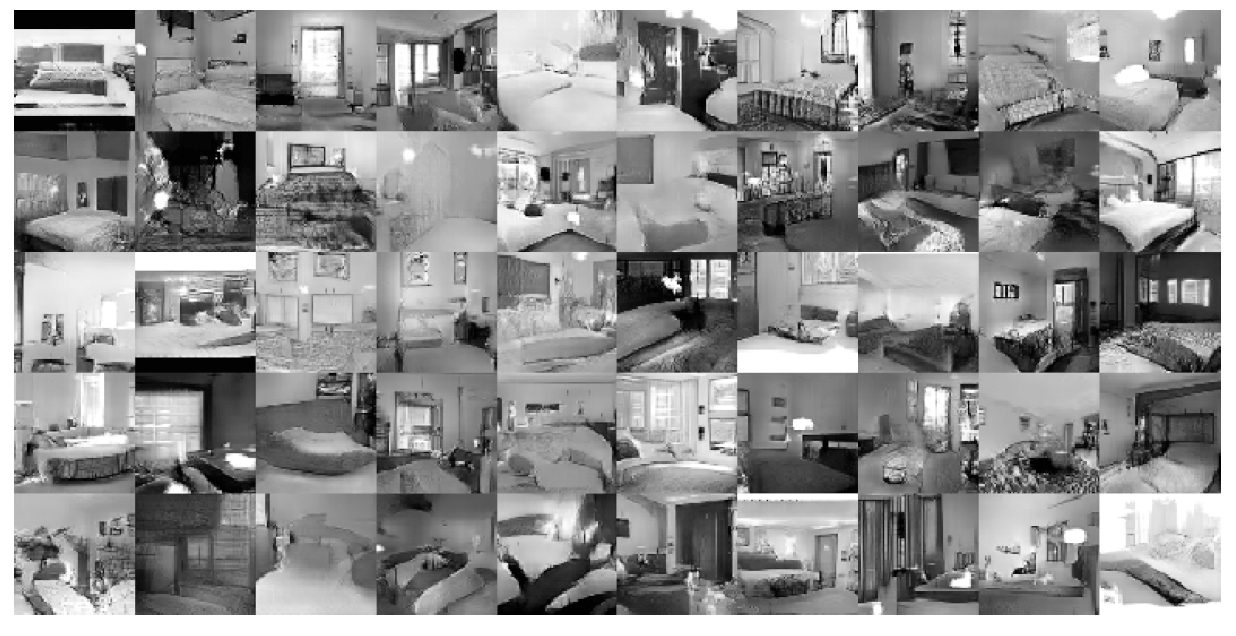
\includegraphics[width=0.6\textwidth]{figures/dcgan.png}

\small DCGAN (Radford 등, 2015)이 만든 침실 이미지. 모두 실제로 존재하지 않는 방이다.
\end{minipage}
\end{center}

아무 입력 없이 (무작위 수에서) 새로운 이미지를 만드는 것도 가능하다.
\textbf{GAN} (Generative Adversarial Network, 2014)은 두 network를 경쟁시킨다.
\begin{itemize}[leftmargin=1.5em]
\item \textbf{생성자(generator)} $G$: 무작위 벡터 $z$를 받아 이미지 $G(z)$를 만든다.
\item \textbf{판별자(discriminator)} $D$: 이미지를 받아 진짜 (훈련 데이터)인지 가짜 ($G$가 만든 것)인지 확률을 낸다.
\end{itemize}
$D$는 진짜와 가짜를 잘 구별하도록, $G$는 $D$를 속이도록 번갈아 학습한다.
위조지폐범과 경찰이 서로 실력을 키우는 것과 같다.
DCGAN은 $G$와 $D$를 CNN으로 만든 GAN이다.
2020년 이후로는 잡음을 조금씩 걷어 내며 이미지를 만드는 \textbf{확산 모델(diffusion model)}이 주로 쓰이며,
문장을 입력하면 그림을 그려 주는 서비스가 널리 쓰이고 있다.

\subsection{자율 주행}\label{sec:driving}

\begin{center}
\begin{minipage}{\textwidth}\centering
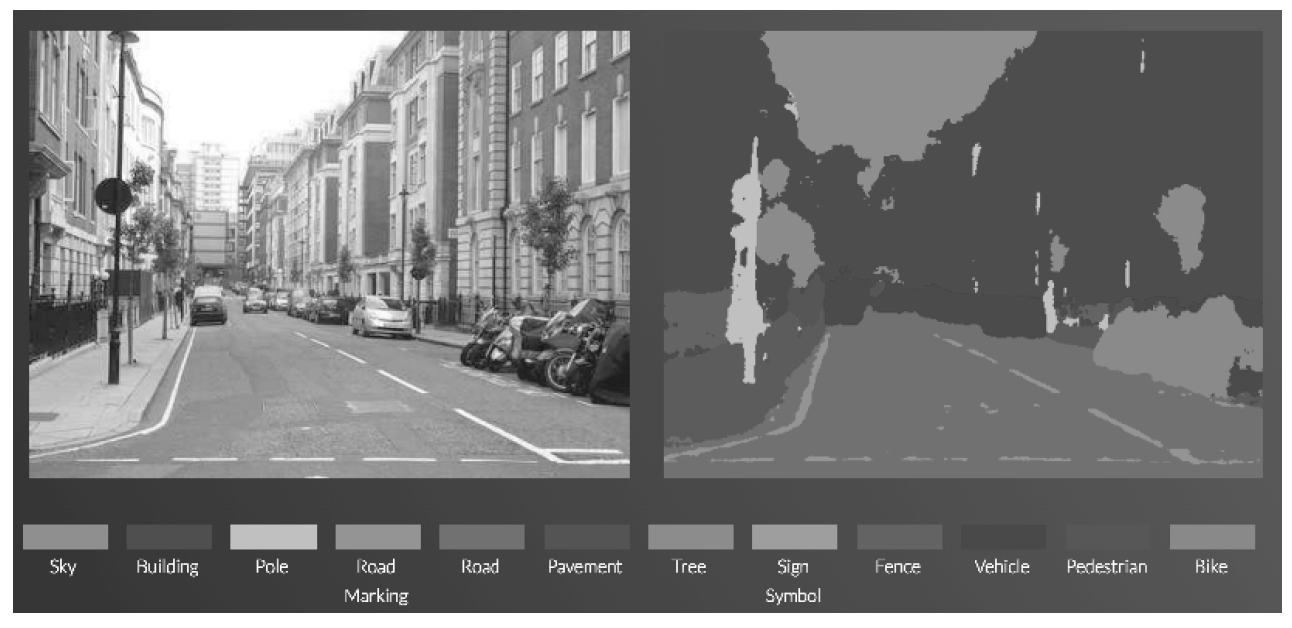
\includegraphics[width=0.6\textwidth]{figures/segnet.png}

\small SegNet (Badrinarayanan 등, 2015)으로 도로 장면을 분할한 예. 도로, 건물, 보도, 나무, 차량 등을 픽셀 단위로 구분한다.
\end{minipage}
\end{center}

자율 주행에는 경로 계획, 센서 처리 등 많은 기술이 필요하지만, 그중에서도 주위 환경을 올바르게 인식하는 일이 가장 어렵고 중요하다.
4.2절의 분할과 4.1절의 검출이 여기에 쓰인다. 날씨, 밤낮, 도로 상황에 상관없이 안정적으로 인식해야 하므로 지금도 활발히 연구되고 있다.

\subsection{강화학습}\label{sec:rl}

사람은 정답을 하나하나 배우지 않아도, 시행착오를 거쳐 스스로 배운다 (예: 자전거 타기).
\textbf{강화학습(reinforcement learning)}은 이렇게 \textbf{보상}을 통해 배우는 방법이다.

\begin{center}
\begin{minipage}{\textwidth}\centering
\begin{tikzpicture}[>=Latex,
  bx/.style={draw,rounded corners=3pt,fill=black!5,minimum width=32mm,minimum height=9mm,font=\small}]
\node[bx] (env) at (0,1.8) {환경 (environment)};
\node[bx,fill=blue!10] (agt) at (0,0) {에이전트 (agent)};
\draw[->,thick] (agt.west) -- ++(-1.2,0) |- node[pos=0.25,left,font=\scriptsize] {행동 $a_t$} (env.west);
\draw[->,thick] (env.east) -- ++(1.2,0) |- node[pos=0.25,right,font=\scriptsize,align=left] {보상 $r_t$,\\다음 상태 $s_{t+1}$} (agt.east);
\end{tikzpicture}
\end{minipage}
\end{center}

\textbf{에이전트}가 환경의 상태를 보고 \textbf{행동}을 하면, 환경이 바뀌고 \textbf{보상}이 주어진다.
에이전트는 앞으로 받을 보상의 합이 커지도록 행동하는 방법을 배운다.
정답 레이블이 아니라 보상이 주어지고, 보상은 행동한 뒤 한참 뒤에 올 수도 있다 (바둑은 끝나야 승패를 안다).

\begin{center}
\begin{minipage}{\textwidth}\centering
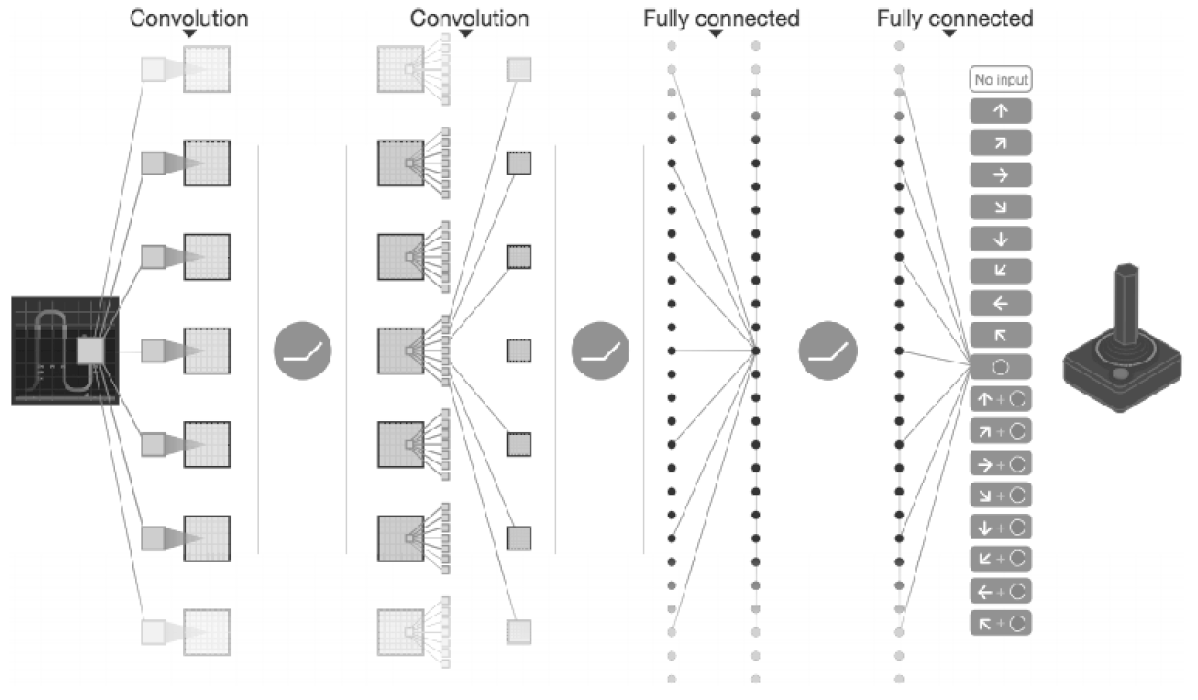
\includegraphics[width=0.6\textwidth]{figures/dqn.png}

\small DQN (Mnih 등, 2015): 게임 화면을 CNN에 넣어, 조이스틱의 각 행동이 얼마나 좋은지 (Q 값)를 출력한다.
\end{minipage}
\end{center}

\textbf{DQN} (Deep Q-Network)은 게임 화면 (최근 $4$프레임)을 CNN에 넣고, 가능한 행동마다
``이 행동을 하면 앞으로 받을 보상의 합''의 추정치를 출력한다. 사람이 게임의 규칙을 알려 주지 않았는데도,
화면과 점수만으로 학습하여 수십 종의 Atari 게임 중 절반 이상에서 사람 수준에 이르렀다.
2016년 이세돌 9단을 이긴 \textbf{AlphaGo}도 CNN과 강화학습을 함께 썼다 (바둑판을 $19\times19$ 이미지로 보고 CNN에 넣었다).

\begin{remarkbox}[그 뒤의 딥러닝 (2017년 이후)]
\begin{itemize}[leftmargin=1.5em]
\item \textbf{Transformer (2017):} 합성곱이나 RNN 대신 \textbf{어텐션(attention)}으로, 입력의 모든 위치가 서로를 직접 참고하게 한 구조이다.
번역을 위해 만들어졌지만 지금은 언어, 이미지, 음성 등 거의 모든 분야의 기본 구조가 되었다.
\item \textbf{큰 언어 모델:} Transformer를 엄청난 양의 문장으로 ``다음 단어 맞히기''를 학습시킨 것이 GPT 같은 언어 모델이고,
2022년 공개된 ChatGPT 이후 대화형 인공지능이 널리 쓰이게 되었다.
\item \textbf{Vision Transformer (2020):} 이미지를 $16\times16$ 조각으로 잘라 단어처럼 Transformer에 넣는다.
데이터가 아주 많으면 CNN 못지않은 성능을 낸다. 그래도 합성곱은 효율이 좋아 지금도 많이 쓰이며, 두 방법을 섞은 모델도 많다.
\end{itemize}
구조는 바뀌었지만 \textbf{계층을 쌓고, 손실을 정하고, 역전파로 기울기를 구해, 경사하강법 (Adam 등)으로 학습한다}는 원리는
이 강의에서 배운 그대로이다. skip connection, 정규화 (배치 정규화의 친척인 layer normalization), 드롭아웃, He 초깃값,
GPU와 혼합 정밀도도 모두 그대로 쓰인다.
\end{remarkbox}

% =================================================
\section{정리}\label{sec:summary}
% =================================================

\begin{keybox}[딥러닝: 정리]
\begin{itemize}[leftmargin=1.5em]
\item $3\times3$ 합성곱 $6$개와 He 초깃값, ReLU, Adam, 드롭아웃을 쓴 DeepConvNet은 MNIST에서 $99\%$가 넘는 정확도를 낸다.
\item 데이터 확장은 정답을 바꾸지 않는 변형으로 훈련 데이터를 늘린다. 훈련 데이터가 적을수록 효과가 크다.
\item 작은 필터를 여러 층 쌓으면 같은 수용 영역을 더 적은 매개변수로 보고 ($25$ vs $18$), 비선형성이 늘고, 문제를 계층적으로 나누어 배운다.
\item 2012년 AlexNet 이후 ImageNet 대회의 오류는 VGG ($3\times3$ 반복), GoogLeNet (인셉션, $1\times1$ 합성곱),
ResNet (skip connection $y=x+F(x)$)을 거치며 사람 수준 아래로 내려갔다.
\item skip connection은 기울기를 그대로 전달하여 $100$층이 넘는 network도 학습할 수 있게 한다.
\item 계산 시간의 대부분은 합성곱 (= 행렬곱)이다. GPU, 데이터 병렬 분산 학습, 16비트 등 낮은 정밀도로 빠르게 한다.
\item CNN은 분류뿐 아니라 검출 (R-CNN, YOLO), 분할 (FCN), 캡션 생성, 스타일 변환, 이미지 생성 (GAN), 강화학습 (DQN)에 쓰인다.
\end{itemize}
\end{keybox}

% =================================================
\section{연습문제}
% =================================================

\begin{enumerate}[label=\arabic*.]

\item DeepConvNet의 Conv4의 패딩을 $2$가 아니라 $1$로 바꾸면 Conv4 다음 풀링의 출력, Conv6 다음 풀링의 출력,
Flatten의 출력 크기는 각각 얼마가 되는가? 첫 번째 Affine 계층의 매개변수 수는 어떻게 바뀌는가?

\item 입력과 출력의 채널이 모두 $C$개일 때, $7\times7$ 합성곱 계층 하나와 $3\times3$ 합성곱 계층 세 개 (패딩 $1$, 스트라이드 $1$)를 비교하라.
(a) 출력 원소 하나의 수용 영역이 같음을 보여라. (b) 편향을 빼고 매개변수 수를 비교하라. (c) $C=64$일 때 각각의 값을 구하라.

\item VGG16의 합성곱 계층의 매개변수 수를 구하라. (첫 블록: $3\to64$, $64\to64$; 둘째: $64\to128$, $128\to128$;
셋째: $128\to256$, $256\to256$ 두 번; 넷째: $256\to512$, $512\to512$ 두 번; 다섯째: $512\to512$ 세 번. 모두 $3\times3$, 편향 포함.)
완전연결 계층 세 개 ($7\cdot7\cdot512\to4096\to4096\to1000$)의 매개변수 수와 비교하라.

\item 입력이 $192$채널이고 $3\times3$ 필터 $128$개를 적용한다. (a) 바로 적용할 때와 (b) $1\times1$ 합성곱으로 $96$채널로 줄인 뒤 적용할 때,
편향을 빼고 매개변수 수를 비교하라. 입력의 공간 크기가 $28\times28$ (패딩 $1$)이면 곱셈 횟수는 각각 얼마인가?

\item 스칼라 블록 $30$개를 생각하자. 일반 network는 $h_{l}=w_l h_{l-1}$, ResNet은 $h_{l}=h_{l-1}+w_l h_{l-1}$이다.
모든 $w_l=0.5$일 때 $\pd{h_{30}}{h_0}$를 각각 구하라. $w_l$이 모두 $0$이면 어떻게 되는가?
이로부터 ``필요 없는 블록은 $F(x)=0$을 배우면 된다''는 말을 설명하라.

\item 미니배치 $B=6$개의 손실이 $\ell_1,\ldots,\ell_6$이고 $L=\frac16\sum\ell_n$이다.
GPU 두 개가 각각 $L_1=\frac13(\ell_1+\ell_2+\ell_3)$, $L_2=\frac13(\ell_4+\ell_5+\ell_6)$의 기울기를 구했다.
$\grad L=\frac12(\grad L_1+\grad L_2)$임을 보여라. 조각의 크기가 $4$개와 $2$개로 다르면 어떻게 합쳐야 하는가?

\item \texttt{float16}은 가수가 $10$비트이다. (a) $1$ 바로 다음으로 나타낼 수 있는 수는? (b) $2048$ 바로 다음 수는?
(c) numpy로 \texttt{np.float16(2048) + np.float16(1)}을 계산하고 결과를 설명하라.
(d) 학습 중 아주 작은 기울기 (예: $10^{-8}$)를 \texttt{float16}으로 바꾸면 어떻게 되는가?

\item 정답 사각형이 $(x,y)=(0,0)$부터 $(4,4)$까지이고, 예측한 사각형이 $(1,1)$부터 $(5,5)$까지이다. IoU를 구하라.
IoU $\ge0.5$를 맞은 것으로 볼 때, 예측 사각형을 정답과 같은 크기로 오른쪽으로만 $d$만큼 옮긴다면 $d$가 얼마까지 맞은 것인가?

\item MNIST의 데이터 확장으로 다음 중 무엇이 적절한가? 이유와 함께 답하라.
(a) $\pm10^\circ$ 회전 (b) 좌우 뒤집기 (c) $180^\circ$ 회전 (d) $\pm2$픽셀 이동 (e) 약간의 굵기 변화
(f) 고양이·개 사진 분류라면 (b)는 어떤가?

\item \texttt{mnist\_deep\_torch.py --n\_train 5000}과 \texttt{--n\_train 5000 --augment}로 학습하고 test 정확도를 비교하라.
1.2절의 표와 함께, 훈련 데이터의 양에 따라 데이터 확장의 효과가 어떻게 달라지는지 설명하라.

\end{enumerate}

\end{document}
